\setlength{\epigraphwidth}{.35\textwidth}
\begin{epigraphs}
\qitem{\textit{Roll up! Roll up for the \\ magical mystery tour!\\
Step right this way!}}%
 {---Magical Mystery Tour,\\ \textsc{The Beatles}}
\end{epigraphs}

Once you become familiar with the fact that the farther out we look in space, the further back we see in time, the Universe is put in a new perspective as it unravels before our eyes. Over the centuries we have come to discover that the Universe is an incredible \emph{place} and, in my personal view, the most amazing aspect is perhaps that it can be remarkably
well described by mathematical means.
In fact, our fair understanding of the Universe has been summarized in the so-called Standard \gls{HBB} model which rests on the following assumptions:
%
\begin{itemize}
\item{On sufficiently large scales the Universe is homogeneous and isotropic (the \gls{CP}).}
\item{\gls{GR} is the theory to describe gravitational interactions on cosmological scales.}
\item{The energy budget of the Universe can be modeled in terms of cosmological fluids with barotropic \gls{EoS}.}
\end{itemize}
%
The model states that the Universe evolved from an initial singularity\footnote{Curiously, the current 
paradigm does not explain the \emph{Big Bang} in the \gls{HBB} (the initial singularity). In fact, the term \gls{HBB} was coined by Fred Hoyle, a supporter of the alternative \emph{steady state} cosmological model.} and it has been
expanding ever since. As a result, the primordial Universe was in a hotter and denser state where 
all species were in thermal equilibrium. This picture is corroborated by three 
fundamental observations: the distance dependent recession of galaxies from which we can infer the 
expansion of the Universe (encoded in the \emph{Hubble law}), the abundances of light elements 
indicating that the Universe went through an hot and dense phase, and the Cosmic Microwave Background (CMB) which is interpreted
as the afterglow of the primeval plasma. 

The theoretical limitations of the \gls{HBB} model, such as the horizon problem or the origin of the
structure seeds, can be overcome within the inflationary framework which postulates a period of 
accelerated expansion in the early Universe, driven by a transient phase of non-zero vacuum energy provided by the potential of a scalar field, the inflaton. As a result, adiabatic and Gaussian perturbations were generated from quantum fluctuations of the inflaton field (as predicted by the simplest inflationary 
scenario).
Then, according to the current paradigm of structure formation, the objects we now observe have
originated from the gravitational collapse of such small perturbations in a homogeneous, expanding 
Universe. The earliest imprint of the primordial inhomogeneities can be observed in the temperature anisotropies of the \gls{CMB}, a snapshot of the Universe at the time of recombination, allowing for 
tight constraints on the space of models. 
This picture of the infant Universe is however distorted by interactions of \gls{CMB} photons with the 
evolving medium through which they are propagating. An important effect is the weak gravitational lensing
of photons trajectories due to the gradient in the gravitational potentials associated to the \gls{LSS} in 
the Universe. Its characteristic effect on the \gls{CMB} anisotropies pattern enables the reconstruction of
lensing maps which probe the total integrated matter distribution out to the last scattering surface, hence
opening a unique window on fundamental physics aspects that affect the structure formation in the 
Universe such as gravity theories, neutrino sector and \gls{DM}.

This Chapter reviews the theoretical framework as well as the key observational tools in cosmology and it
is split in three main sections. Sec.~\eqref{FLRW_cosmo} describes the modeling of the 
background Universe together with its constituents, and it sketches how structures form and evolve 
from the initial conditions set by inflation. The physics of the \gls{CMB} temperature and polarization 
anisotropies is discussed in Sec.~\eqref{sec:cmb}, while the last part, Sec.~\eqref{sec:lensing}, is dedicated to 
the weak gravitational lensing as a cosmological probe, focusing on the case of \gls{CMB} lensing.



\section{FLRW Cosmology}
\label{FLRW_cosmo}

\subsection{Zeroth-order cosmology: the Background Universe}
\label{Cosmo_background}
The \gls{CP} is meant to be statistical, that is the Universe is \emph{on average} homogeneous (invariant
under spatial translations, i.e. the cosmological properties are the same throughout) and isotropic 
(invariant under spatial rotations, i.e. there are no preferred directions). Homogeneity does not imply 
isotropy and viceversa; however, if we accept the Copernican Principle, according to which we do not live 
in a particular position in the Universe, then isotropy guarantees the homogeneity of the whole Universe 
\citep{Ellis1975}. While homogeneity can hardly be tested, the isotropy
is well established by observations of the \gls{CMB} \citep{Bennett1996}, the X-ray background \citep{Boughn2002a}, and the spatial distribution of galaxies \citep{Marinoni2012}. For  a discussion on cosmologies that do not rely on the Copernican Principle, 
we refer the reader to \citet{Clarkson2012}. \\
The assumption of the \gls{CP} allows us to define a universal time variable, the \emph{cosmic time}, and to
represent the Universe by a time-ordered sequence of three-dimensional spatial slices, each of which is
homogeneous and isotropic. If we also consider the Universe not to be static, as Hubble observations suggest, then the \gls{FLRW} metric is the most general 
metric describing an expanding spacetime. When expressed in the \emph{comoving} spherical coordinate system $x^i=(\chi, \theta,\phi)$ it has the following form:
%
\begin{align}
\label{eq:flrw}
\diff s^2 &= -c^2\diff t^2 + a^2(t)\gamma_{ij}\diff x^i \diff x^j\\
& = -c^2 \diff t^2 + a^2(t) \bigl[\diff \chi^2 + f^2_K(\chi) (\diff \theta^2 + \sin^2{\theta}\diff \phi^2)\bigr]\\
& = -c^2 \diff t^2 + a^2(t) \bigl[\diff \chi^2 + f^2_K(\chi) \diff\Omega^2\bigr],
\end{align}
%
where the \emph{scale factor} $a(t)$ (normalized to $a(t_0)=1$ today) encodes the expansion of the 
Universe and the \emph{comoving transverse distance}\footnote{Also referred to as the \emph{metric} or 
\emph{proper distance}.} can take - depending on the spacetime curvature - the following forms:
%
\be
f_K(\chi) = 
\begin{cases}
\sin{\chi} & \quad {\rm{if}} \, K = 1 \\
\chi & \quad {\rm{if}} \, K = 0 \\
\sinh{\chi} & \quad {\rm{if}} \, K = -1, \\
\end{cases}
\ee
%
Physical size are related to the comoving ones through $d_{\rm p} = a(t)\chi$.  
The physical velocity of an object is $v = \dot{d}_{\rm p} = \dot{a}\chi + a\dot{\chi} \equiv Hd_{\rm p} + 
v_{\rm pec}$, where we defined the \emph{Hubble parameter} $H \equiv \frac{\dot{a}}{a} = \frac{\diff a}{a\diff t}$ that describes the expansion history of the Universe and the dot denotes proper time derivative, i.e. $\dot{} \equiv \frac{\partial}{\partial t}$. It is customary to normalize its present 
day value, $H_0$, in terms of the dimensionless parameter $h$ as $H_0 = 100\,h$ km/s/Mpc.  
The Hubble parameter naturally introduces a  characteristic expansion timescale given by $H^{-1}$ 
which corresponds to the age of the Universe at that time\footnote{It is roughly the time in which the 
scale factor doubles.}. Similarly to distances we can define the \emph{conformal time} as 
$\diff \eta = \diff t / a(t)$: with this definition, the Hubble parameter becomes $\mathcal{H} \equiv \diff\ln{a}/
\diff\eta = aH$. \\
An important consequence of the Universe expansion is that light gets stretched. A photon emitted at a 
time $t_{\rm{em}}$ with wavelength $\lambda_{\rm{em}}$ will be observed at a time $t_{\rm{obs}}$ with a 
wavelength $\lambda_{\rm{obs}}$ given by
%
\be
\frac{a(t_{\rm{obs}})}{a(t_{\rm{em}})} = \frac{\lambda_{\rm{obs}}}{\lambda_{\rm{em}}} \equiv 1 + z,
\ee
%
where the \emph{cosmological redshift} $z$ was defined. 

\myparagraph{Distances}
Distances in cosmology are not uniquely defined. The \emph{comoving distance} between us and a source at redshift $z$ is given by
%
\be
\label{eq:comdist}
\chi = \int_t^0  \frac{c\diff t'}{a(t')} = \int_a^1\frac{c\diff a'}{a'^2H(a')} = \int_0^z \frac{c\diff z'}{H(z')}.
\ee
%
In a flat universe ($K = 0$), the comoving transverse distance is simply equal to the comoving distance 
$\chi$. Note also that both $f_K$ and $\chi$ distances are \emph{not} observable.\\
The causality structure of the Universe is determined by the photons trajectories: in \gls{FLRW} cosmologies
we can define the \emph{particle horizon} $\chi_{\rm{ph}}$  as the greatest comoving distance from which
light could have reached us by now (assuming the Big Bang at $t_i=0$)
%
\be
\label{eq:ph}
\chi_{\rm{ph}} = \int_0^t \frac{c\diff t'}{a(t')} = \int_0^a \frac{c\diff a'}{a'^2H(a')} = \int_z^{\infty} \frac{c\diff z'}{H(z')}.
\ee
%
It is straightforward to see that $\chi_{\rm{ph}}(t)=c\eta$. Regions which are separated by a distance larger
than the horizon size $d_{\rm{ph}}(t) = a(t)\chi_{\rm{ph}}(t)$ cannot be in causal contact. It is worth to stress
that the particle horizon $\chi_{\rm{ph}}$ and Hubble radius $(aH)^{-1}$ are roughly the same for a \gls{FLRW} cosmology but are generally different.\footnote{Strictly speaking, this is true if the energy budget of the Universe is dominated by a \emph{pressure-less dust} component.} The Hubble radius is the (comoving) distance
over which particles can travel in the course of one expansion time. So, if two regions are separated by 
$\lambda > \chi_{\rm{ph}}$, they have \emph{never} communicated, whereas if  
$\lambda > (aH)^{-1}$, then they are not in causal contact \emph{now}. \\
Cosmologists commonly make use of standard candles, i.e. objects with known luminosity $L$ (like
the Type-Ia SN), and  standard rulers, i.e. sources with a known physical size $l$ (such as the
fluctuations in the \gls{CMB}). These probes allow us to define the \emph{luminosity distance} 
$D_L$ as the distance to a standard candle with measured flux $F = \frac{L}{4\pi D^2_L(z)}$ as:
%
\be
\label{eq:lumdist}
D_L \equiv \sqrt{\frac{L}{4\pi F}} = \frac{f_K(\chi)}{a} = (1+z)f_K(\chi),
\ee
%
and the \emph{angular diameter distance} as the distance to an object of dimension $l$ subtending and
angle $\delta\theta$:
%
\be
\label{eq:angdist}
D_A \equiv \frac{l}{\delta\theta} = a(t)f_K(\chi) = \frac{f_K(\chi)}{1+z}.
\ee
%
From Eq.~\eqref{eq:lumdist} and \eqref{eq:angdist} we see that angular diameter and luminosity distances are 
not independent but they are related through the Etherington's distance-duality relation 
\citep{Etherington1933}:
%
\be
\label{eq:etherington}
D_L = (1+z)^2D_A.
\ee
%
The redshift dependence of the three distance measures $f_K(\chi)$, $D_L$, and $D_A$ is shown in 
\eqref{fig:dist} for a flat cosmology with (solid lines) and without dark energy (dashed lines) in the form of
a cosmological constant $\Lambda$, a cosmic component with vacuum energy-like features that we introduce below, hypothesized to source the late-time cosmic acceleration. As can be seen, all the distances are enlarged by the presence of   
$\Lambda$. \\

\begin{figure} %1
\centering % \begin{center}/\end{center} takes some additional vertical space
\includegraphics[width=0.7\textwidth]{Chapter1/Images/dists}
\caption{Different distance measures for a flat cosmology with cosmological constant $\Omega_{\Lambda}
=0.7$ (solid lines) and matter-only (dashed lines). \label{fig:dist}}
\end{figure}

\myparagraph{Friedmann Equations}
So far the discussion focussed on the symmetries of the spacetime and led us to the definition of the \gls{FLRW}
metric. The dynamics of the background Universe, described by the time evolution of $a(t)$, can be worked
out by relating the metric to the energy content of the Universe. This is achieved via the  \gls{EFE} 
%
\be
\label{eq:EFE}
G_{\mu\nu} \equiv R_{\mu\nu}-\frac{1}{2}g_{\mu\nu}R = 8\pi G T_{\mu\nu}+\Lambda g_{\mu\nu}, 
\ee
%
where $G_{\mu\nu}$ and $R_{\mu\nu}$ are the Einstein and Ricci tensors computed from the metric, $R=R_{\mu}^{\mu}$ is the Ricci scalar, and $T_{\mu\nu}$ is the \gls{SET} which
describes the energy content of the Universe. In order to allow for static solutions ($\dot{a}=0$) of the \gls{EFE}, which were considered to describe our Universe before Hubble's discovery of recession of galaxies,
Einstein introduced a \emph{cosmological constant} term $\propto \Lambda g_{\mu\nu}$ whose presence
does not spoil the Bianchi identity. In principle this term could be equivalently added to the l.h.s., and be interpreted as a geometrical feature of the spacetime, or to the r.h.s. of 
Eq.~\eqref{eq:EFE} as a contribution to the \gls{SET} 
$T_{\mu\nu}^{\rm{vac}}=\frac{\Lambda}{8\pi G}g_{\mu\nu}$. The physical interpretation is still debated 
but a non-zero cosmological constant provides nowadays the simplest explanation for the cosmic acceleration.  Homogeneity and isotropy also constrain the form of the \gls{SET} to be the one of a perfect fluid at rest in 
comoving coordinates:
%
\be
\label{eq:SET}
T^{\mu}_{\nu} = (\rho+P)u^{\mu}u_{\nu} - P\delta^{\mu}_{\nu},
\ee
%
where $u^\mu$ is the relative four-velocity between the fluid and the observer, while $\rho=\rho(t)$ and 
$P=P(t)$ are the \emph{energy density} and \emph{pressure} in the rest-frame of the fluid. In this case,
the time-time component of the \gls{EFE} can be solved to yield the time evolution of the expansion rate $H$
%
\be
\label{eq:FE_exp}
H^2 \equiv \biggl( \frac{\dot{a}}{a} \bigg)^2 = \frac{8\pi G}{3}\rho + \frac{\Lambda}{3} - \frac{K}{a^2},
\ee
%
while the spatial components of the \gls{EFE} reduce to a single expression for the acceleration:
%
\be
\label{eq:FE_acc}
\frac{\ddot{a}}{a} = -\frac{4\pi G}{3}(\rho + 3P) + \frac{\Lambda}{3},
\ee
%
where $\rho = \sum_a\rho_a$ and $P=\sum_a P_a$ are the total energy density and pressure of the 
Universe. Eqs~\eqref{eq:FE_exp} and \eqref{eq:FE_acc} are usually called the \emph{Friedmann equations},
from which we see that the total energy density of a flat Universe ($K=0$) corresponds to the
\emph{critical density} $\rho_{\rm{crit}}$ defined as 
%
\be
\label{eq:critdens}
\rho_{\rm{crit}} = \frac{3H^2}{8\pi G}.
\ee
%
Note that it depends on time and its present value $\rho_{\rm{crit}}^{0}$ is approximately $10^{-27}$ kg/m$^3$.
The critical density is useful to define dimensionless density parameters for the different species as 
$\Omega_i(t) = \frac{\rho_i(t)}{\rho_{\rm{crit}}(t)}$. Cosmological fluids are assumed to be 
\emph{barotropic}, that is, their pressure is given as an explicit function of their energy density so that we 
can define the fluid \gls{EoS} $w$ as $P = w(\rho)\rho$ and the \emph{sound
speed} as $c_s^2 = \delta P/\delta\rho$.  From the conservation of the \gls{SET}, $\nabla^{\mu}T_{\mu\nu}=0$,
we find that the time evolution of the energy density obeys
%
\be
\label{eq:cont}
\dot{\rho} + 3H(\rho+P)=0.
\ee
%
The continuity equation applies separately to each species as long as their particle number is conserved
and their energy exchange can be neglected. Then, for a constant $w$, the energy density scales as
$\rho \propto a^{-3(1+w)}$, while for a time-dependent EoS $w(a)$, one has to solve the following
integral:
%
\be
\label{eq:densev}
\rho \propto \exp \biggl(-3\int_0^a \frac{\diff a'}{a'}[1+w(a')] \biggr).
\ee
%
With these scalings and the dimensionless densities, we can rewrite Eq.~\eqref{eq:FE_exp} as
%
\be
\label{eq:h_z}
H^2(z) = H_0^2 \bigl[ \Omega_{\rm r0}(1+z)^4 + \Omega_{\rm m0}(1+z)^3 + \Omega_{\rm K0}(1+z)^2 + \Omega_{\Lambda} \bigr].
\ee
%
It is useful to classify the different species according to their contribution to pressure as:
\begin{itemize}
\item{\textbf{Matter}: All sources for which the internal pressure is much smaller than the energy density,
$|P| \ll \rho$, like the case of a gas of non-relativistic particles (where the mass $m$ is much bigger than
the momentum $p$). Baryons (i.e. nuclei and electrons) and \gls{DM} represent two dust-like species.
In this case $w\approx 0$ and the energy density is diluted by cosmic expansion as $\rho \propto a^{-3}$.}
\item{\textbf{Radiation}: The term refers to species for which the pressure is about a third of their energy
density, $P=\frac{1}{3}\rho$ so that $w=\frac{1}{3}$ and $\rho \propto a^{-4}$. 
This is the case of a gas of relativistic particles (for which $m\ll p^2$), like photons, neutrinos and massive
species while still relativistic.}
\item{\textbf{Dark Energy}: Even though the term indicates a plethora of models which source the cosmic
acceleration, here we consider a cosmological constant which exerts a negative 
pressure $P=-\rho$ so that $w = -1$. In this case the energy density is constant and does not feel the 
cosmic dilution, $\rho \propto a^0$. The vacuum energy predicted by quantum field theory provides a 
natural explanation for \gls{DE}, however its expected density $\rho_{\rm{vac}}$ is off by $\approx 120$ orders 
of magnitude with respect to the observed one.}
\end{itemize}

\myparagraph{Cosmic Inventory}
What we have sketched above is just a framework that employs few parameters which are not fixed 
\emph{a priori}. Deciding which values the cosmological parameters should assume for our Universe 
relies on observational constraints. A combination of cosmological probes, including observations of the
\gls{CMB}\footnote{From an historical point of view, \gls{CMB} measurements provide the tightest constraints.}, the 
\gls{LSS} (such as the \gls{BAO} and galaxy clusters), and the Type-Ia SN magnitude-redshift relation has 
now placed strong constraints on the cosmological parameters. The emerging picture is an almost flat 
Universe mainly composed of \emph{dark} ingredients we cannot yet theoretically account for.
Observations show that the Universe is filled with radiation ($\Omega_{\rm r}$), matter 
($\Omega_{\rm m}$), and \gls{DE} ($\Omega_{\Lambda}$) with an EoS that remarkably resembles the one 
of a cosmological constant $w_{\Lambda}\approx - 1$. Ordinary baryonic matter can account for just 5\%
of the total budget, while most of the matter content is in the form of a clustering dark component which
appears to interact only gravitationally or weakly at most. The most popular candidate for \gls{DM} is a
Weakly Interacting Massive Particle (WIMP), an hypothetical elementary particle. WIMPs are generally
referred to as Cold Dark Matter (CDM) because their velocity (or thermal pressure) is small so that they behave as a  non relativistic fluid. \gls{DM} properties have a pivotal role in structure formation: if CDM is dominant, then larger structures form by accreting smaller structures. Relativistic  species are represented by photons (mainly in the form of \gls{CMB}) and neutrinos. Summing up all the ingredients we have 
$\Omega_K = 1- \Omega_{\rm{r0}} - \Omega_{\rm{m0}} - \Omega_{\Lambda} \simeq 0$.
As can be seen in Fig.~\eqref{fig:cosmic_history}, depending on the species that is the most abundant we can identify three epochs in the cosmic history: the \emph{radiation dominated era} ($a \propto \eta$), the \emph{matter domination era} ($a \propto \eta^2$)
and the \emph{\gls{DE} dominated era} ($a \propto 1/\eta$ ). The transitions between the three eras take 
place at $a_{\rm{eq}} = \frac{\Omega_{\rm r0}}{\Omega_{\rm m0}} = 2.93\times10^{-4}$ and 
$a_{\Lambda} = \frac{\Omega_{\rm m0}}{\Omega_{\Lambda}} = 0.46$ (corresponding to $z_{\rm{eq}}=
3410$ and $z_{\Lambda} = 1.18$, respectively). This concordance model goes under the name of \gls{LCDM} and the main constituents contribution to the total $\Omega$, as well as other cosmological parameters that will be defined later on, is listed in Table~\eqref{tab:densities}. 
%
\begin{table}[t]
\centering
\begin{tabular}{ccccc}
\toprule
\midrule
\multicolumn{5}{ c }{Densities} \\
\textbf{Parameter} & $\Omega_{\rm b}$  & $\Omega_{\rm cdm}$  & $\Omega_{\Lambda}$  & $\Omega_{\rm r}$ \\
\textbf{Value} & $0.0490^{+0.0005}_{-0.0005}$  & $0.2642^{+0.0005}_{-0.0005}$  & $0.685^{+0.013}_{-0.013}$  & $\simeq 9.2\times 10^{-5} $  \\
\midrule
\multicolumn{5}{ c }{Others} \\
\textbf{Parameter}& $H_0$ & $n_s$ & $10^9A_s$ & $\tau$  \\
\textbf{Value}&$67.31^{+0.96}_{-0.96}$ & $0.9655^{+0.0062}_{-0.0062}$ & $2.198^{+0.076}_{-0.085}$ & $0.078^{+0.019}_{-0.019}$\\
\midrule
\bottomrule
\end{tabular}
\caption{Parameters of the vanilla \gls{LCDM} cosmology computed from the 2015 baseline Planck likelihoods for the \gls{CMB} temperature power spectra plus low-$\ell$ polarization data (referred to as \emph{Planck} TT+lowP in \citet{PlanckCollaboration2015b}).}
\label{tab:densities}
\end{table}
%
\begin{figure} %2
\centering % \begin{center}/\end{center} takes some additional vertical space
\includegraphics[width=0.7\textwidth]{Chapter1/Images/dens}
\caption{Cosmic history of the Universe. The blue curve is the scale factor as a function of conformal time, obtained by solving the Friedmann equation, while the dashed lines represent the radiation, matter and cosmological constant densities as function of conformal time. Adapted from \citet{Pettinari2016}.\label{fig:cosmic_history}}
\end{figure}
%
\myparagraph{Dark Energy or Modified Gravity?}
The accelerated expansion of the Universe, first \emph{discovered} in 1998 \citep{Riess1998,Perlmutter1999}, 
has raised great interest
both in the cosmology and the physics community as a whole: the mechanism behind the acceleration
still remains elusive and it represents one of the main scientific drivers of the upcoming experimental 
efforts. Even though a cosmological constant is consistent with the current observations, it is essential
to consider alternatives from a phenomenological perspective. Over the last years a classification scheme
has emerged to distinguish between physical scenarios that source the cosmic acceleration: namely
the \emph{Dark Energy} and \emph{Modified Gravity} (MG) models. Naively, DE models
modify the r.h.s. of \gls{EFE} by adding an additional component to the \gls{SET}, while \gls{MG} models alter the l.h.s. of
\gls{EFE}, hence modifying the Einstein-Hilbert action (i.e. they change GR itself). 
Giving a thorough overview of all existing theories is far beyond the purposes of this thesis, 
but we refer the reader to \citet{Silvestri2009,Clifton2012} for complete reviews on the topic.  
Here we just sketch the main ideas behind the two approaches and, following the prescription of 
\citet{Joyce2016},
we distinguish between \gls{DE} and \gls{MG} by means of the \emph{strong equivalence principle} (SEP):  any
theory which obeys the SEP is classified as \gls{DE}, while any theory which violates it as MG. Heuristically,
the SEP forbids the presence of fifth forces.\\
The most natural extension to the cosmological constant paradigm is that is a dynamical field 
(dubbed \gls{DE}) which relaxes to its present value via some mechanism \citep{Wetterich1988, Ratra1988}.
This idea is at the base of many different theoretical implementations, that all share the presence of a
degree of freedom that  drives the background cosmological evolution. Perhaps the most obvious
generalization of the canonical scalar field with a potential is the following:
%
\be
S = \int \diff^4 x \sqrt{-g} \Lambda^4 K(X),
\ee
%
where we defined $X\equiv -\frac{1}{2\Lambda^4}(\partial \phi)^2$ and $K(X)$ is an arbitrary function:
these models are usually referred to as $k-$essence \citep{Chiba2000,Armendariz-Picon2000}. Similar to
the canonical case, if the field has an homogeneous profile $\phi=\phi(t)$, these models behave as a 
(slightly more complicated) perfect fluid with EoS parameter $w$ given by
%
\be
w = \frac{K}{2XK_{,X} - K}.
\ee
%
The background expansion history can be reproduced by a suitable choice of the functional form for $K$.
It is worth to notice that in $k-$essence models the field perturbations do not propagate luminally but
with a sound speed given by
%
\be
c_s^2 = \frac{K_{,X}}{K_{,X} + 2XK_{,XX}},
\ee
%
allowing for significant differences with \gls{LCDM} in the structure formation.\\
On the other hand, modifications to GR lead to new physics on small scales \citep{Lue2004}, 
introducing new degrees of freedom in the gravity sector. Since these new particles mediate a fifth-force,
\gls{MG} theories must develop some \emph{screening mechanism} in order to evade the very constraining 
local tests of gravity, like the ones on Solar System scales. In Ch.~\eqref{Sec:Models} we will discuss a specific model of \gls{MG} named $f(R)$, where the standard Einstein-Hilbert action gets modified by the presence of a generic function of the Ricci scalar.

\subsection{First-order cosmology: the Perturbed Universe}
\label{sec:Cosmo_pert}
The assumption of homogeneity and isotropy significantly simplifies the mathematical description of
the Universe as a whole, however it just holds when looking at scales larger than approximately $100$ 
Mpc. On smaller scales observations of the galaxies distribution and of the \gls{CMB} fluctuations 
anisotropy pattern tell us that the Universe is far from being homogeneous, showing a complex structure and rich hierarchy composed by stars, globular clusters, galaxies, galaxy clusters, filaments and voids. 
These structures are thought to be originated from primordial fluctuations through gravitational instability. 
As we mentioned already, the Universe is not homogeneous even on larger scales, as it is seen in the anisotropies of the \gls{CMB}. Here we sketch the theory of cosmological perturbations, first introduced by \citet{Lifshitz1946}; classic literature on the subject is by \citet{Kodama1984, Ma1995} and the review by \citet{Bernardeau2002}.

\myparagraph{Relativistic perturbations}
The basic idea is to consider small perturbations around the \gls{FLRW} metric and the perfect fluid \gls{SET} and 
couple them through \gls{EFE}; after subtracting the background, we are left with\footnote{We remind that
here the dot represents proper time derivative $\dot{} \equiv \frac{\partial}{\partial t}$, while the prime
denotes conformal time derivative $' \equiv \frac{\partial}{\partial \eta}$.}
%
\be
\label{eq:pertEFE}
\delta G_{\mu\nu} = 8\pi G \delta T_{\mu\nu}.
\ee
%
If the perturbations are small, we can perform a perturbative expansion on both sides and keep the 
linear terms. Assuming the background metric to be spatially flat, the most general form for the metric fluctuations can be written in conformal coordinates as
%
\be
\label{eq:pertFLRW}
\diff s^2 = a^2(\eta)\{-(1+2\phi)\diff \eta^2 + 2B_i\diff x^i\diff\eta + [(1-2\psi)\delta^K_{ij} + E_{ij}]\diff x^i \diff x^j\}.
\ee
%
The perturbations $\psi$ and $\phi$ are scalars, while $B_i$ and $E_{ij}$ can be split into scalar, vector
and tensor parts as:
%
\begin{align}
B_i &= \underbrace{\partial_i B}_{\rm{scalar}} + \underbrace{\hat{B}_i}_{\rm{vector}} \quad \text{with} \quad \partial^i \hat{B}_i = 0\\
E_{ij} &= \underbrace{\partial_{\langle i}\partial_{j\rangle} E}_{\rm{scalar}} + \underbrace{\partial_{(i} \hat{E}_{j)}}_{\rm{vector}} + \underbrace{\hat{E}_{ij}}_{\rm{tensor}} \quad \text{with} \quad \partial^i \hat{E}_i = \partial^i\hat{E}_{ij} = 0,
\end{align}
%
where 
%
\begin{align}
\partial_{\langle i}\partial_{j\rangle} E &\equiv  \left( \partial_i\partial_j - \frac{1}{3}\delta_{ij}\nabla^2 \right) E, \\
\partial_{(i} \hat{E}_{j)} &\equiv  \frac{1}{2}\left( \partial_i \hat{E}_j + \partial_j \hat{E}_i \right). 
\end{align}
%
Scalar fluctuations are induced by density inhomogeneities and exhibit gravitational
instability leading to structure formation. Vector modes are strongly
suppressed by cosmic expansion. Tensor perturbations are an important prediction of the inflationary 
paradigm and describe gravitational waves. Scalar-Vector-Tensor (SVT) decomposition is powerful 
because it decouples Einstein equations for scalar, vectors and tensor modes, whose evolutions can be 
thus treated separately. However, the problem of relativistic perturbation theory is the gauge redundancy in GR: 
the way to deal with such issues is either to fix a gauge (i.e., a coordinate system) in order to make any
two of the four scalar functions $\phi$, $\psi$, $B$ and $E$ vanish or work in terms of \emph{gauge-invariant} 
perturbations.\footnote{Here, $B$ and $E$ refer to the scalar components of the metric fluctuations and should not be confused with the $E$- and $B$-modes decomposition of the \gls{CMB} polarization that we will discuss in Sec.~\eqref{sec:cmb_prim}.} The most common  gauge-invariant linear combinations of these function are the so called
\emph{Bardeen's potentials} \citep{Bardeen1980,Mukhanov1992}:
%
\be
\Phi \equiv \phi -\frac{1}{a}[a(B-E')]' \quad \text{and} \quad \Psi \equiv \psi + \frac{a'}{a}(B-E').
\ee
%
On the r.h.s. of Eq.~\eqref{eq:pertEFE} we can perturb the \gls{SET} to linear order like:
%
\begin{align}
\label{eq:pertSET}
\delta T^0_0 &= -\delta\rho \\ 
\delta T^0_i &= (\bar{\rho} + \bar{P})v_i \\ 
\delta T^i_j &= \delta P\delta^i_j + \Pi^i_j,
\end{align}
%
where bar denotes background quantities and $\Pi^i_j$ is the anisotropic stress tensor.
If we substitute the metric from Eq.~\eqref{eq:pertFLRW} into \gls{EFE} and keep only the linear order 
perturbations, we find the \emph{gauge-invariant} perturbation equations \citep{Mukhanov2005}:
%
\begin{align}
\label{eq:pertEFE2}
\nabla^2\Psi - 3\mathcal{H}(\Psi' + \mathcal{H}\Phi) &= 4\pi Ga^2\delta T^0_0 \\
\partial_i(\Psi'+\mathcal{H}\Phi) &= 4\pi G a^2\delta T^0_i \\
\Bigl [\Psi''+\mathcal{H}(2\Psi+\Phi)' + (2\mathcal{H}'+\mathcal{H}^2)&\Phi +\frac{1}{2}\nabla^2(\Phi-\Psi) \Bigr]\delta_{ij} - \frac{1}{2} \partial_i\partial_j(\Phi-\Psi) = -4\pi G a^2 \delta T^i_j.
\end{align}
%
These equations can be derived without imposing any gauge conditions and they are valid in an arbitrary coordinate system. 

\myparagraph{Conformal Newtonian gauge}
Here we work in the \emph{conformal Newtonian gauge} (or the \emph{longitudinal 
gauge}), defined by choosing $B = E = 0$ in  Eq.~\eqref{eq:pertFLRW}: in this coordinate system the metric takes the form 
%
\be
\label{eq:pertFLRW_conf}
\diff s^2 = a^2(\eta)[-(1+2\Phi)c^2\diff\eta^2 + (1-2\Psi)\delta_{ij}\diff x^i \diff x^j].
\ee
%
Note that this metric is similar the usual weak-field limit of GR about Minkowski space: in the Newtonian
limit, $\Phi$ plays the role of the gravitational potential, i.e. it governs the dynamics of non-relativistic
objects, while the combination (Weyl potential) $\Psi_{\gamma}\equiv (\Psi+\Phi)/2$ determines the null
geodesics, i.e. light propagation. Going to Fourier space, the perturbation equations in 
Eq.~\eqref{eq:pertEFE2} expressed in the conformal Newtonian gauge for a mode with comoving
wavenumber $k$ become:
%
\begin{align}
\label{eq:pertEFE3}
k^2\Psi + 3\mathcal{H}(\Psi' + \mathcal{H}\Phi) &= -4\pi Ga^2\delta\rho \\
k^2(\Psi'+\mathcal{H}\Phi) &= 4\pi G a^2 (\bar{\rho}+\bar{P})\theta \\
\Psi''+\mathcal{H}(2\Psi'+\Phi') &+ \frac{3}{2}\mathcal{H}^2(1+w)\Phi + \frac{k^2}{3}(\Psi-\Phi) = 4\pi G \delta\rho \\
k^2(\Psi-\Phi) &= 12\pi G a^2 (\bar{\rho}+\bar{P}) \sigma,
\end{align}
%
where $\theta \equiv \partial_i v^i = \nabla \cdot \mathbf{v}$ is the velocity divergence and $\sigma$ is the
anisotropic stress, i.e. the trace-free part of $T_{ij}$. 
The source terms on the r.h.s. are meant to be the sum over all the relevant matter-energy components:
in the absence of anisotropic stress\footnote{In reality, neutrinos develop anisotropic stress after neutrino decoupling (i.e. they do not behave like a perfect fluid), so that $\Phi$ and $\Psi$ differ from each other 
by about 10 \% between the neutrino decoupling and the matter-radiation equality; during matter 
domination neutrinos contribution is negligible and the two potentials approach each other.} $\Phi = \Psi$.
Conservation of the \gls{SET}, $\nabla_{\mu}T^{\mu\nu}=0$, yields the two following equations (for $\mu=0$ and $\mu=i$) in the conformal
Newtonian gauge \citep{Ma1995}
%
\begin{align}
\label{eq:pertSETeq}
\delta' &= -(1+w) (\theta - 3\Psi') - 3 \mathcal{H} (c_s^2 - w)\delta \\
\theta' &= -\mathcal{H}(1 - 3w)\theta - \frac{w'}{1+w}\theta + \frac{c_s^2}{1+w}k^2\delta + k^2\Phi - k^2\sigma,
\end{align}
%
which are the relativistic generalization of the continuity and Euler equation.\\
The equations derived above are fully relativistic and provide an adequate description of perturbations
on scales larger than the Hubble radius and for relativistic fluids (like photons and neutrinos).

 Looking at
the relative size between the perturbation wavenumber and Hubble radius, we can distinguish two 
regimes: $k \ll \mathcal{H}$ called super-Hubble modes, and $k \gg \mathcal{H}$, referred to as 
sub-Hubble modes\footnote{Note that in literature super- and sub-Hubble modes are often (improperly) called super-and sub-horizon modes. See the discussion on the differences in 
Sec.~\eqref{Cosmo_background}}. In the regime when we are deep within the Hubble radius, we can take 
the non-relativistic limit of the perturbed \gls{EFE} in order to greatly simplify the description of perturbations.
However, these equations are nonlinear and several efforts have been made in the past to find 
approximate solutions for a wide range of scales and redshifts: the most straightforward approach goes
under the name of Standard Perturbation Theory, while other approaches are the so called Renormalized
Perturbation Theory and the Effective Field Theory. The efforts aimed at improving the perturbations 
description towards nonlinear scales are essential for a successful comparison of theory and data in the 
light of upcoming \gls{LSS} surveys such as Euclid, \gls{LSST}, \gls{DESI}, and \gls{WFIRST}.

\myparagraph{Scales smaller than the Hubble radius}
Assuming a \gls{DM} dominated Universe, on \emph{sub-Hubble scales} the linearized\footnote{We assume 
the densities and velocities to be small, i.e. $\delta \ll 1$ and $v \ll c$.} Poisson, continuity and
Euler equations for matter perturbations read:
%
\begin{align}
\label{eq:pertEFEnewt}
\nabla^2\Phi &= \frac{3}{2}\Omega_{\rm m}(\eta) \mathcal{H}^2(\eta)\delta \\
\delta' + \theta &= 0 \\
\mathbf{v}' + \mathcal{H}\mathbf{v} &= - \nabla\Phi.
\end{align}
%
Combining them, one finds a second-order linear differential equation for the linear density contrast
%
\be
\label{eq:lineardelta}
\delta'' + \mathcal{H}\delta' - \frac{3}{2}\mathcal{H}^2\Omega_{\rm m}\delta = 0.
\ee
%
In this equation only time derivatives appear, hence solutions can be factorized into a spatial and 
time-dependent solutions, associated to a growing and decaying mode; in general we can write
%
\be
\delta(\mathbf{x},t) = D_+(\eta) A(\mathbf{x}) + D_-(\eta) B(\mathbf{x}),
\ee
%
where $A(\mathbf{x})$ and $B(\mathbf{x})$ are two arbitrary functions describing the initial density field, while $D_{\pm}$ are the growth and decay functions. In a matter dominated Universe $\mathcal{H} = 
2/\eta$, so that 
%
\be
D_+(\eta) = \eta^2 \quad \text{and} \quad D_-(\eta) = \eta^{-3}.
\ee
%
The explicit time-dependence makes clear why the two solutions are known as growing and decaying 
modes: the relevant mode for structure formation is the former, while the latter quickly fades away.
It is customary to normalize the solution by the growing mode today, such that we define the \emph{growth factor} as :
%
\be
\label{eq:growth}
D(a) \equiv \frac{D_+(a)}{D_+(a_0=1)}.
\ee
%

\myparagraph{Scales greater than the Hubble radius}
What does happen when the perturbation is much larger then the Hubble radius? 
Assuming that the pressure depends only on the energy density and the EoS $w$ is a constant, then we have $c_s^2 = w$ (which is valid both for matter and radiation). In this case the first two lines of 
Eq.~\eqref{eq:pertEFE2} can be combined to yield 
%
\be
\Phi'' + 3\mathcal{H}(1+c_s^2)\Phi' = 0,
\ee
%
for which $\Phi =$ const is the growing solution. Note that this super-Hubble solution is independent on 
$w$ as long as it is constant; in particular, the gravitational potential is frozen outside the Hubble radius
(during radiation and matter domination). It is also possible to show that a frozen potential at large 
scales implies that the density contrast $\delta \approx -2\Phi =$ constant as well. Density perturbations
are therefore simply proportional to the curvature perturbation: this is a key ingredient for setting the 
initial conditions and to link inflation with perturbation evolution.

\myparagraph{Transfer function, power spectra and galaxy bias}
So far we just described the qualitative behavior of perturbations in an expanding Universe and we have 
seen that it depends on (i) whether the perturbation mode is larger or smaller than the Hubble radius and
(ii) on the species that dominates the cosmic energetic budget. Let's summarize the main results here. \\
The gravitational potential $\Phi$ is constant when the modes are outside the horizon: if they cross the
horizon during the radiation era, they start to oscillate and their amplitude decreases as $a^2$,
while during the matter era the potential is constant on all scales. 
During the radiation domination the radiation fluctuations are constant on super-Hubble scales, while they
oscillate if $k \gg \mathcal{H}$; in the matter era, the subhorizon fluctuations in the radiation density
 oscillate with constant amplitude around a shifted equilibrium point. For CDM, we have that perturbations on super-Hubble scales remain frozen both during radiation
and matter domination: this means that the properties of such modes are preserved from the early
Universe. If the perturbations enter the horizon during the radiation-dominated epoch, they grow 
logarithmically, $\delta_{\rm m} \propto \ln a$, while the growth is a power-law ($\delta_{\rm m} \propto a$)
if the horizon is crossed during the matter domination. When the Universe becomes dominated by \gls{DE},
perturbations stop growing.
Baryons behavior is somewhat different because they are coupled with photons through Compton
scattering prior to the decoupling at $z\sim 1100$, so that we can treat the photons and baryons as a 
single fluid. On sub-Hubble scales they oscillate with decreasing amplitude together with the photons,
while after the decoupling, since the effective baryons pressure drops to approximately zero, their 
oscillations are not supported by photons, enabling gravitational collapse (if the perturbation scale is 
below the \emph{Jeans length}).
To account for all the interactions between different components and the effects at play on all scales, such
as causality, one can define a \emph{transfer function} $T(k)$ as \citep{Eisenstein1998}
%
\be
\label{eq:trans_func}
T(k) \equiv \frac{\delta(k,z=0)}{\delta(k,z=\infty)}\frac{\delta(0,z=\infty)}{\delta(0,z=0)},
\ee
%
which can be defined for each species and, by construction, $T \to 1$ for $k \to 0$. In order to derive 
$T(k)$ one has to numerically solve the Boltzmann equation (as done by the Code for Anisotropies in the Microwave Background (\texttt{CAMB}) \citep{Lewis2000a} or the Cosmic Linear Anisotropy Solving System (\texttt{CLASS}) \citep{Lesgourgues2011}) but there also can be found fitting formulae in literature, see 
\cite{Bardeen1986,Eisenstein1998}. Then the (matter) power spectrum at a given time
$\langle |\delta(\bm{k},z)|^2\rangle$ is 
proportional to the square of the transfer function and the growth factor, multiplied by the initial power 
spectrum $P_{\rm ini}(k)$ set by inflation (as we will see in Sec.~\eqref{sec:inflation})
%
\be
\label{eq:pk}
P_{\delta\delta}(k,z) = D^2(z)T^2(k)P_{\rm ini}(k).
\ee
%
The normalization of the matter power spectrum is determined from observations and it is common 
practice to measure the variance of the smoothed overdensity field over a comoving scale $R$ 
(usually taken to be 8 Mpc/$h$) at present as 
%
\be
\sigma^2_R = \int \frac{\diff^3k}{(2\pi)^3}P_{\delta\delta}(k,z=0)|W_R(k)|^2, 
\ee
%
where $|W_R(k)|^2$ is a window function which usually is a top-hat filter in real space.
 
However, we need
to bare in mind that our observations rely on using galaxies to trace the overall matter distribution and as 
such, they provide a biased picture of matter clustering: the statistical relation between the dark and 
luminous matter distribution is described by the \emph{galaxy bias} $b$. The idea that galaxy formation  is 
enhanced in dense environment was introduced by \citet{Kaiser1984}\footnote{In order to explain the 
stronger correlation function of galaxy clusters with respect to the galaxies one.} and generalized by \citet{Bardeen1986,Sheth1999} in the peak-background split framework. \cite{Fry1993} then proposed that
galaxies $\delta_g$ trace matter distribution $\delta$ through a non-linear transformation, 
$\delta_g(\bm{x}) = \mathcal{F}[\delta(\bm{x})]$, which can be Taylor-expanded to obtain the so-called
\emph{local\footnote{This is because the galaxy overdensity at some position $\bm{x}_1$ is not affected
by the density displaced in $\bm{x}_2$, otherwise the bias is said to be non-local and the coefficients $b_i$ would carry spatial dependence.} biasing scheme}:
%
\be
\label{eq:bias}
\delta_g(\bm{x}) = \sum_{i}^{\infty} \frac{b_i}{i!}\delta^i(\bm{x}).
\ee
%
The perturbative expansion is usually halted at the linear order and one finds $\delta_g = b_1 \delta$, so 
that the galaxy power spectrum reads as $P_{gg}(k) = b_1^2 P_{\delta\delta}(k)$. At small 
scales the linear bias relation breaks down because of nonlinear structure formation and acquires 
non-local features like the scale dependence, even though for $k\lesssim 0.01 h/$Mpc the linear relation should hold. 
Measuring the galaxy bias of the high-$z$ \gls{DSFG} will be a central topic of Ch.~\eqref{ch:xc1} and~\eqref{ch:xc2}.  

A semi-analytical model that has proven useful to address both nonlinear clustering and galaxy bias is the 
\emph{halo model}, developed from the pioneering work of \citet{Neyman1952} and then formalized by 
\citet{Scherrer1991,Seljak2000}  (see \citet{Cooray2002} for a comprehensive review). The basic idea is 
that at late times all the matter distribution is contained only in virialized \gls{DM} objects called \emph
{halos}, and the galaxy distribution can be modeled by an appropriate scheme for placing galaxies in these 
\gls{DM} halos. The fundamental assumption of the model is that the average halo properties, such as 
its density profile and its galaxy content, only depend on the halo mass. As a consequence, the total 
matter power spectrum splits into two terms, $P_{\delta\delta}(k) = P_{\delta\delta}^{\rm 1h}(k)+P_{\delta\delta}^{\rm 2h}(k)$ where $P_{\delta\delta}^{\rm 1h}$ is the 1-halo term describing correlations on small 
scales between mass within the same halo and $P_{\delta\delta}^{\rm 2h}$ is the 2-halo term arising from 
large-scale correlation of matter in different halos. 


\subsection{Setting the initial conditions: Inflation}
\label{sec:inflation}
The \gls{HBB} scenario we depicted so far is a remarkably simple model that allows us to describe 
the Universe both at the background and at the perturbation level. Nonetheless, the model is unable to 
explain the following theoretical and observational problems which we summarize briefly here below. It is beyond the scope of this thesis to give a comprehensive description of the physics of the very early Universe, and our discussion is targeted to define the power spectrum of scalar perturbations generated during inflation. For a more complete discussion, we refer the reader to \cite{Mukhanov2005}.

\textbf{Flatness problem.} The spatial curvature is observationally constrained to be negligible (|$\Omega_K| 
\ll 1$) \citep{PlanckCollaboration2015b}. Moreover, from the Friedmann equation, one can show that 
$\Omega_K$ grows with time, so that the spatial curvature becomes vanishingly small as time runs 
backward. This means that a flat geometry is an unstable solution and if the density today is close to the critical 
one, as observations suggest, it had to be much more so in the past, requiring unnatural initial conditions 
(\emph{fine tuning} problem). 

\textbf{Horizon problem.} Any correlations between regions separated by a distance greater than the particle 
horizon cannot be naturally explained by the standard model. However, the \gls{CMB} appears to be 
isotropic (to $10^{-5}$ precision, see Sec.~\eqref{sec:cmb}) over much bigger scales\footnote{Barbara
Ryden in her cosmology textbook \citep{Ryden2003} compares this situation to "\emph{inviting 20.000 people to a potluck
dinner and they all bring potato salad}".}.

\textbf{Monopoles problem.} Most extensions of the standard model of particle physics, like the Grand
Unification Theory (GUT), predict the creation of magnetic monopoles which would be produced during
transition phases in the early Universe. However, no monopole relics have been observed to date.

\textbf{Structure problem.} Despite the solid perturbation theory formalism developed in the sections above,
we lack of a mechanism that explains the formation of the primordial seeds that eventually lead to the 
structure formation via gravitational collapse.

As we already mentioned, these shortcomings are all connected to the Universe initial conditions and
can be solved by postulating the existence of a period of accelerating expansion in the early Universe,
the so-called \emph{cosmic inflation} \citep{Guth1981,Starobinsky1982,Linde1982}. 
The effect of the cosmic acceleration predicted by the inflationary models\footnote{The term inflation refers to a \emph{mechanism} rather than a \emph{theory} of the early Universe.} is to hugely increase 
the size of the Universe, washing out any curvature and stretching the geometry of the Universe in a way
that it becomes spatially flat, hence solving the flatness problem. Moreover cosmic inflation solves the 
horizon problem by connecting regions that, in the standard HBB model, would be causally disconnected.
This can be achieved if the comoving Hubble radius at the beginning of inflation is larger than the largest
scale observable today, i.e. the current Hubble radius.\footnote{It is worth to stress that it is not the 
accelerated expansion that solves the horizon problem: the causal connection is established 
\emph{before} the inflationary epoch and then inflation simply puts these regions out of reach again.}
Inflation also solves the apparent monopole paradox by completely diluting their density, so that
there may be an arbitrarily small number of relics in the observable Universe. Inflationary models also 
predict an almost scale-invariant power spectrum of primordial density perturbations, which serve as
initial conditions to the process of structure formation, as we explain in some more detail below. \\
For the cosmic expansion to be accelerated, Eq.~\eqref{eq:FE_acc} requires the Universe to be dominated 
by a species of negative pressure which fulfills:
%
\be
\ddot{a} > 0 \Leftrightarrow \rho + 3P < 0 \Leftrightarrow w < -\frac{1}{3}.
\ee
%
This can be achieved if we consider a Universe in which a cosmological constant is dominant at early 
times. Then, since $w = -1$, the background expansion is de Sitter and the scale factor increases 
exponentially in time, $a(t) \propto e^{Ht}$. At the end of inflation, the duration of which can be "tuned" in order
to solve the problems discussed above, the cosmic acceleration comes to an end and the cosmological 
constant decays into a thermal mix of elementary particles, leading to a radiation dominated Universe.
This process is the so-called \emph{reheating} and thereafter the Universe can evolve according to the 
standard HBB model.\\
Over the years a plethora of inflationary models have emerged on the market (for a comprehensive 
review of the \emph{zoology} see, for instance, \cite{Martin2014}), and they all share the
presence of one or more real scalar fields $\phi_i$, with associated potentials $V_i(\phi_i)$, which 
drive the accelerated expansion. The particles corresponding to these fields are called \emph{inflatons}.\\
To sketch how single-field inflation works, consider a Universe dominated by an homogeneous scalar field 
$\phi$ that behaves as a perfect fluid with 
%
\begin{align}
\rho_{\phi} &= \frac{1}{2}\dot{\phi}^2 + V(\phi) \\
p_{\phi} &= \frac{1}{2}\dot{\phi}^2 - V(\phi).
\end{align}
%
Then, the equation of motion of the scalar field is given by 
%
\be
\ddot{\phi} + 3 H\dot{\phi} + \frac{\diff V}{\diff \phi} = 0,
\ee
%
which corresponds to an oscillator equation for a scalar field experiencing the damping of the Hubble 
expansion. Since the inflaton dominates the energy budget, the Friedmann equation becomes
%
\be
H^2 = \frac{8\pi G}{3}\biggl[\frac{1}{2}\dot{\phi} + V(\phi) \biggr] - \frac{K}{a^2}, 
\ee
%
and we immediately notice that if $a$ grows by many orders of magnitude then the term $K/a^2 \to 0$,
leading to a spatially flat universe. The sought-after accelerated expansion can be achieved under the
\emph{slow-roll condition} that is, $\dot{\phi}^2 \ll V(\phi)$. In this case the $w_{\phi}\approx -1$ so that 
the scale factor grows as $a \propto e^{Ht}$, where $H(t) \approx$ const for slowly varying potentials. 
Several potentials can be tailored in order to satisfy the slow-roll condition and it is common practice to 
parametrize them with the two \emph{slow-roll parameters} defined as 
%
\be
\epsilon \equiv \frac{\diff}{\diff t} \Bigl ( \frac{1}{H}\Bigr) = - \frac{\dot{H}}{H^2} \quad \text{and} \quad \eta 
\equiv \frac{\dot{\epsilon}}{H\epsilon}.
\ee
%
If both $\{\epsilon, \eta\} \ll \mathcal{O}(1)$, then slow-roll inflation takes place.\\ 
Cosmic inflation also provides a mechanism to generate primordial density fluctuations 
\cite{Starobinsky1982, Hawking1982, Bardeen1983}. 
These primordial fluctuations are the result of the microscopic quantum vacuum fluctuations in the inflation
field that, during inflation, get stretched out by the accelerated expansion and imprinted on super-horizon
scales. Eventually, the density fluctuations reenter the horizon and serve as initial conditions for the 
growth of structure in the Universe. The requirement $\epsilon \ll 1$ translates into an approximate 
time-translation invariance of the background, so that primordial fluctuations generated during inflation are 
expected to have the same variance on all scales. We can define the power 
spectrum of the \emph{ primordial comoving curvature perturbation}, $\mathcal{R} = \Psi - \frac{1}{3} \frac{\delta\rho_{\rm tot}}{\bar{\rho}_{\rm tot} + \bar{p}_{\rm tot}}$, as
%
\be
\label{eq:prim_pow}
\mathcal{P}_{\mathcal{R}}(k) = \frac{k^3P_{\mathcal{R}}(k)}{2\pi^2} = A_s \biggl( \frac{k}{k_*} \biggr)^{n_s-1},
\ee
%
where the scale invariance\footnote{The exact scale invariance is achieved if $H$ and $\phi$ are constant
in time during inflation; however this is only an approximation as we know that the inflaton must have a 
dynamics otherwise the inflation continues forever.} is usually expressed in terms of the \emph{scalar 
spectral index} $n_s$. $A_s$ is the \emph{amplitude of the primordial scalar fluctuations} evaluated
at the the pivot scale $k_*$ (commonly taken to be 0.05 $h/$Mpc or 0.02 $h/$Mpc).
The scalar spectral index is linked to the slow-roll parameters through $n_s = 1 - 6\epsilon + 2\eta$ and
recent measurement from \textit{Planck}, in combination with other experiments, measured a value of
$n_s = 0.9655 \pm 0.0062$ \citep{PlanckCollaboration2015b}, excluding $n_s =1 $ at more than 
$8\sigma$. The primordial power spectrum appearing in Eq.~\eqref{eq:pk} can be taken to be $P_{\rm ini}(k)=2\pi^2k^{-3}\mathcal{P}_{\mathcal{R}}(k) = P_{\mathcal{R}}(k)$. 
 Another robust and model-independent 
prediction from the inflationary mechanism is the production of a stochastic background of primordial
gravitational waves that is also expected to be nearly scale invariant. Similarly to the case of scalar 
perturbations in Eq.~\eqref{eq:prim_pow}, we define the power spectrum of tensor fluctuations as 
%
\be
\mathcal{P}_t(k) = A_t \biggl( \frac{k}{k_*} \biggr)^{n_t}.
\ee
%
The tensor and scalar fluctuations are related through the tensor-to-scalar ratio 
$r \equiv \frac{\mathcal{P}_t(k_*)}{\mathcal{P}_{\mathcal{R}}(k_*)}$, which represent a valuable probe
of the inflation physics since it directly sets the energy scale for inflation as
%
\be
V^{1/4} \approx \Bigl ( \frac{r}{0.01} \Bigr )^{1/4} 10^{16}\, \text{GeV}. 
\ee
%
The statistics of primordial perturbations is usually characterized in terms of power spectra, however 
they are just one of the infinite $n$-point functions that describe a random field (see Sec~\eqref{sec:RF}). 
For a Gaussian random field these moments can be written in terms of the 2-point function, i.e. the power
spectrum, while for generic random fields this is not true. Higher-order moments carry 
information about the nonlinear physics of the early Universe and, in particular, about the interactions of
the inflaton. Since the inflationary potential is expected to be very flat, the interactions are expected to be 
very small as well. The deviations of primordial fields from a perfectly Gaussian distribution are known as
\emph{non-Gaussianities} (NG); for a pedagogical review on primordial NG from inflationary models we
refer the reader to \cite{Chen2010}. In this context, \gls{CMB} has become one of the best laboratory to study
NG: statistics like the bispectrum (3-point function) and the trispectrum (4-point function) of the \gls{CMB} can
be used to assess the level of primordial NG (and possibly its shape) on different cosmological scales 
and to disentangle it from the one induced by secondary anisotropies and systematic effects 
\citep{Bartolo2010}. To date, the tightest constraints on NG, and on the inflationary epoch in general, are provided by the latest release of \textit{Planck} collaboration \citep{Ade:2015ava}.

\section{Cosmic Microwave Background}
\label{sec:cmb}
The \gls{CMB} was first fortuitously discovered in 1965 by Arno Penzias and Robert
Wilson while working on long-distances radio communications at the Bell Laboratories\footnote{The first 
observations of the \gls{CMB} were actually made in the forties by McKellar \citep{McKellar1940}, who studied the population of excited rotational states of CN molecules in interstellar absorption lines.} 
\citep{Penzias1965}. It represents the first compelling evidence of the \gls{HBB} model proposed by 
Gamow in the forties \citep{Gamow1946} and it is interpreted as being the leftover radiation of the 
primordial plasma - when the Universe was in a hot and dense state - and as such it is characterized  
by a blackbody spectrum at a temperature of about 3K . 
In the early Universe ($10^3 \lesssim z \lesssim 10^8$), protons ($p$), electrons 
($e^-$) and photons ($\gamma$) were tightly coupled into the so called photo-baryonic plasma.
Protons and electrons interact through Coulomb scattering while photons were coupled to electrons via
Compton scattering (Thomson scattering in the low-energy limit), maintaining the three species in thermal
equilibrium through:
%
\begin{align}
\label{eq:cmb_reacs}
p+e^- &\leftrightarrow H+\gamma \\
e^- + \gamma &\leftrightarrow e^- + \gamma.
\end{align}
% 
The thermal equilibrium allows to define a single temperature $T$ for the photo-baryonic fluid, common 
to all the species. The cosmic  expansion causes the Universe to cool down, hence diluting the 
density of photons with energy greater than the hydrogen ionization energy, $E_{\gamma} > 13.6$ eV. 
The effect is to spoil the balance in the reaction in Eq.~\eqref{eq:cmb_reacs}, leading to $p+e^-\to H+\gamma$: this process is dubbed \emph{recombination} and happens at a redshift $z_{\rm rec} \simeq 1400$ (corresponding to $T_{\rm rec} \simeq 3900$K), when approximately 50\% of the free electrons 
were captured by protons into hydrogen atoms.\footnote{In reality the temperature of recombination is 
much smaller than the binding energy of the hydrogen atom, $T_{\rm rec} \ll 13.6$ eV. This is mainly because
the photon-to-baryon ratio is very large, $\approx 10^9$, and the high-energy tail of the photons 
distribution is still efficient in breaking hydrogen atom down to lower temperatures.} The Universe 
becomes transparent to radiation only when the photon mean free path is larger than the Hubble radius 
at that time, i.e. when the electron-photon interaction rate $\Gamma(z)$ is similar to the Hubble 
expansion rate: $\Gamma(z_{\rm dec}) \simeq H(z_{\rm dec})$, where we defined the \emph{decoupling}
redshift. Observation suggest that the previous condition is satisfied at $z_{\rm dec} = 1089.90\pm 0.23$ 
\citep{PlanckCollaboration2015b}.

Thermal equilibrium ensures that the \gls{SED} of the \gls{CMB} photons is well described by Planck's 
statistics
%
\be
\label{eq:cmb_SED}
B_{\nu}(T) = \frac{2hv^3}{c^2}\frac{1}{e^{\frac{h\nu}{k_BT}}-1},
\ee
%
where $h$ is the Planck constant, $\nu$ is the frequency and $k_B$ is the Boltzmann constant. The first
measurement of the \gls{CMB} energy spectrum over the frequency range $\nu \in [50,650]$ GHz has 
been made in the early nineties with the \gls{FIRAS} instrument \citep{Mather1994} on board of the  \gls{COBE} satellite, showing that it has a Planckian shape with an equivalent 
brightness temperature of about $T = 2.725 \pm 0.001$ \citep{Fixsen1996}.

 Measurements of the 
\gls{CMB} blackbody spectrum can tightly constrain energy injections in the primordial plasma. While
any energy injection prior to $z_{\rm therm} \approx 10^7$ would have time to be thermalized\footnote{With the term \emph{thermalization} we refer to the process that erases possible spectral distortions of
the CMB in the early Universe, hence attempting to restore full thermodynamic equilibrium.}, a posterior
energy release would cause a distortion of the black-body spectrum \citep{Danese1982,Burigana1991}.
Two main types of \emph{spectral distortions} are usually distinguished, the $y$- and $\mu$-type 
distortions. The former type arises at $z \lesssim \text{few}\times 10^3-10^4$ when the Compton
process ceases to be extremely efficient and is characterized by a
constant temperature decrement at low and an increment at high frequencies. The latter type of distortion 
forms at times when the Compton process can still achieve full kinetic equilibrium
with the electrons ($z \lesssim \text{few} \times 10^5$), and the CMB spectrum reaches a Bose-Einstein 
distribution with non-zero chemical potential $\mu$. 
After the constraining \gls{FIRAS} measurements on the spectral distortions, $|\mu | < 9 \times 10^{-5}$ and $|y|<1.5\times 10^{-5}$ at 95\% confidence level, the subject of spectral distortion has recently attracted a renewed theoretical attention \citep{Chluba2012,Chluba2014} especially in light of upcoming satellite missions aiming at improving such measurements such as the \gls{PIXIE} \citep{Kogut2011} and \gls{COrE}. 

\subsection{Primary anisotropies}
\label{sec:cmb_prim}
\myparagraph{Temperature power spectrum}
The \gls{CMB} photons carry information about the density, velocity and gravitational potential inhomogeneities 
imprinted by inflation to the photo-baryonic plasma. These tiny inhomogeneities in the plasma source the tiny departures from the average temperature, the so called \emph{primary} \gls{CMB} temperature anisotropies\footnote{Here, the term \emph{anisotropies} refers to the temperature fluctuations as function of the \gls{LOS} and should not be confused with the notion of \emph{statistical anisotropic} random fields.}, which provide
a snapshot of the Universe at the time of decoupling. 

The \gls{CMB} temperature sky can be decomposed into 
%
\be
\label{eq:cmbsky}
T^{\rm obs}(\nver) = T_0 \biggl[1  + (\bm{\beta}\cdot\nver) + \frac{T(\nver)}{T_0} \biggr], 
\ee
% 
where $T_0$ is the mean blackbody temperature, $\bm{\beta} = \bm{v}/c$ is the Earth proper velocity 
vector with respect to the \gls{CMB} rest frame, and $T(\nver)$ is the \gls{CMB} temperature fluctuation field. 
The intrinsic temperature anisotropies are of the order $\Theta\equiv  \frac{\Delta T}{T_0} 
\sim \mathcal{O}(10^{-5})$,
approximately two orders of magnitude smaller than the kinematic dipole signal due to the Doppler 
boosting. Let us stress that Eq.~\eqref{eq:cmbsky} is just an approximation as it does not include the 
contribution from 
foreground emissions $F_{\nu}(\nver)$ that has to be taken into account when dealing with real data. 

The intrinsic stochastic nature of the quantum fluctuations during inflation prevents us from developing
a theory that exactly predicts the pattern of $T(\nver)$, nonetheless the problem can be properly
tackled from a statistical point of view. We start by decomposing our scalar \gls{CMB} temperature field 
$T(\nver)$ in spherical harmonics $Y_{\ell m}(\nver)$, a frequency-space orthonormal 
basis for representing functions defined over the sphere (see Sec.~\eqref{sec:harmanalysis}), such that\footnote{The 
monopole $\ell=0$ and dipole $\ell=1$ are left out, see Eq.~\eqref{eq:cmbsky}.}
%
\be
\Theta(\nver) = \sum_{\ell=2}^{\infty} \sum_{m=-\ell}^{\ell} a_{\ell m}^{T}Y_{\ell m}(\nver), \quad \text{where}
\quad a_{\ell m}^{T} = \int \diff\Omega\, \Theta(\nver)Y^*_{\ell m}(\nver),
\ee
%
and the angular scale $\theta$ and multipole moment $\ell$ are related by $\theta \sim 1/\ell$.\\
The randomness of the initial conditions does not allow us to predict any particular $a_{\ell m}^T$ 
coefficient, but different theories tell us about the distribution from which they are drawn.
Considering $T(\nver)$ to be a Gaussian real-valued random field, then the harmonic coefficients 
are complex Gaussian random variables which satisfy the following relations:
%
\begin{align}
\label{eq:cmbprop}
&\langle a_{\ell m}^T \rangle = 0, \, \forall \{\ell, m \}, \\
&\text{Isotropy} \Rightarrow \langle a_{\ell m}^T a_{\ell' m'}^{T*} \rangle = \delta^K_{\ell\ell'}\delta^K_{mm'}C_{\ell}^{TT},\\
&T(\nver)\in \mathbb{R} \Rightarrow a_{\ell-m}^T = (-1)^m a_{\ell m}^{T*},
\end{align}
%
where $\langle\cdot\rangle$ denotes an average over an ensemble of sky realizations and $C_{\ell}^{TT}$ 
is the \emph{angular power spectrum}, i.e. the variance of the $a_{\ell m}^T$. The CP guarantees that the 
covariance matrix of the harmonic coefficients is diagonal, otherwise the off-diagonal components would
introduce a preferred direction in the sky, hence breaking the statistical isotropy of the temperature field.
Then, the diagonal part of the covariance matrix, $C_{\ell}^{TT}$ contains all the statistical information of 
the \gls{CMB} field. Even if we are allowed to observe only one realization of the stochastic field, we can
construct a power spectrum estimator from a single realization of the sky by replacing the ensemble 
average in Eq.~\eqref{eq:cmbprop} with the spatial (sample) average, i.e. averaging over the $2\ell+1$ 
$m$-samples\footnote{It is possible to prove that a random field is \emph{ergodic} if it can be described by 
a Gaussian statistics and if its power spectrum is continuous \citep{Adler2007}.}. The commonly used power 
spectrum estimator reads as (see Sec.~\eqref{sec:ps_est})
%
\be
\hat{C}_{\ell}^{TT} = \frac{1}{2\ell+1}\sum_m |a_{\ell m}^{T}|^2,
\ee
%
which is unbiased, i.e. $\langle\hat{C}_{\ell}^{TT}\rangle = C_{\ell}^{TT}$, and described by a chi-square
distribution with $2\ell+1$ d.o.f., while the diagonal covariance is given by 
%
\be
\label{eq:cmb_CV}
(\Delta \hat{C}_{\ell})^2 = \frac{2}{2\ell+1}C_{\ell}^{2}.
\ee
%
This result is known as \emph{cosmic variance}. 
The harmonic space formalism can easily be linked to the configuration
space 2-point correlation function $C^{TT}(\theta)\equiv\langle T(\nver)T(\nver')\rangle$ as\footnote{Sometimes labelled as $w(\theta)$, especially in clustering analysis. } 
%
\be
\label{eq:c2cl}
\begin{split}
C^{TT}(\theta) &= \sum_{\ell m}\sum_{\ell'm'} \underbrace{\langle a_{\ell m}^Ta_{\ell' m'}^{T*} \rangle}_{\delta^K_{\ell\ell'}\delta^K_{mm'}C_{\ell}^{TT}} Y_{\ell m}(\nver) Y_{\ell' m'}^*(\nver')  \\
&= \sum_{\ell} C^{TT}_{\ell} \underbrace{\sum_{m} Y_{\ell m}(\nver) Y_{\ell m}^*(\nver)}_{\frac{2\ell+1}{4\pi}P_{\ell}(\nver\cdot\nver')}\\
&= \sum_{\ell}\frac{2\ell+1}{4\pi}C_{\ell}^{TT}P_{\ell}(\nver\cdot\nver'),
\end{split}
\ee
%
where $\nver\cdot\nver'=\cos{\theta}$ and we used the addition theorem for spherical harmonics to 
express the product of $Y_{\ell m}$ in terms of the Legendre polynomials $P_{\ell}(x)$.

We now seek a theoretical framework that allows us to compute the observables given a set of 
cosmological parameters. The CMB temperature angular spectrum can be computed via the 
\gls{LOS} integration method (see \cite{Seljak1996} for an extensive discussion) as
%
\be
\label{eq:cmb_cl}
C_{\ell}^{TT}= 4\pi\int \diff\log{k}\, \mathcal{P}_{\mathcal{R}}(k) |\Theta_{\ell}^T(k,\eta_0)|^2.
\ee
%
This method elegantly connects the physics at recombination with the projection effects by writing the 
photon transfer functions $\Theta_{\ell}^T(k,\eta)$ as a time integral of a set of source functions 
$S_T(k,\eta)$ multiplied by the spherical Bessel functions $j_{\ell}(x)$:  
%
\be
\Theta_{\ell}^T(k,\eta_0) = \int_0^{\eta_0} \diff\eta S_T(k,\eta)j_{\ell}[k(\eta_0-\eta)].
\ee
%
The temperature source term can be split as\footnote{Neglecting the contribution from polarization.} \citep{Lesgourgues2014}
%
\be
\label{eq:cmb_ST}
S_T(k,\eta) = g\biggl(\frac{1}{4}\delta_{\gamma}+\Phi\biggr) + e^{-\tau}(\dot{\Phi}+\dot{\Psi}) + \frac{g}{k}\theta_b,
\ee
%
where $\tau(\eta)$ is the optical depth $\tau=\int$ for a photon emitted at time $\eta$ and received at $\eta_0$ and
$g(\tau)=-\dot{\tau}e^{-\tau}$ is the visibility function which peaks around the last scattering epoch at 
$\eta=\eta_*$. The first term in Eq.~\eqref{eq:cmb_ST} contains the intrinsic temperature fluctuations $\frac{1}{4}\delta_{\gamma}$ and the gravitational redshift term $\Phi$ responsible for the Sachs-Wolfe effect\footnote{The Sachs-Wolfe term is sometimes considered to be the sum $\frac{1}{4}\delta_{\gamma}$ 
and $\Phi$.}.
The second term in $S_T(k,\eta)$ is sourced by the time evolution of the gravitational potentials and gives
rise to the so-called \gls{iSW} effect that, in the case of standard \gls{GR} where the two potentials are 
equal, reduces to $S_T^{\rm iSW} \to -2e^{-\tau}\dot{\Phi}$ (see Sec.~\eqref{sec:cmb_secanip}). Doppler effects induced by the peculiar motion of the photo-baryonic fluid are given by the $\theta_b$ term.

By looking at the temperature power spectrum (normalized as $\mathcal{D}^{TT}_{\ell}=\frac{\ell(\ell+1)}{2\pi}C_{\ell}^{TT}$) shown in Fig.~\eqref{fig:cmb_spectra}, we can appreciate a rich structure and distinguish three main features sourced by few physical effects: 
\begin{enumerate} 
\item{the \emph{Sachs-Wolfe 
plateau} at $\ell \lesssim 100$, that almost faithfully traces the initial conditions (which have not had enough time to evolve on such big scales);} 
\item{a prominent peak around  $\ell \sim 100$ followed by a series of \textit{acoustic 
peaks}, produced by modes of the density perturbations which have experienced one or more acoustic oscillations (driven by the competing action of gravity and pressure) before last scattering;}
\item{an overall damping of the spectrum for $\ell \gtrsim 1000$ caused by photon diffusion at recombination (\emph{Silk damping}) and the fact that these small-scale fluctuations have a size comparable to the width of the last scattering surface (it is rather a \emph{layer} than a surface).}
\end{enumerate}

\myparagraph{Polarization power spectra}
\gls{CMB} photons can be, and in fact are, polarized (at the 10\% level). \gls{CMB} polarization represents
an invaluable source of information on inflation and on the late-time evolution of the Universe, like 
reionization and structure formation (through the lensing effects).

Light polarization is commonly described in terms of the \emph{Stokes parameters} $I, Q, U,$ and $V$.
As we have seen, the \gls{CMB} total intensity $I$ has a blackbody spectrum along the \gls{LOS}, 
while the parameters $Q$ and $U$ describe the linear polarization and $V$ describes the circular 
polarization (which is expected to vanish for the \gls{CMB}). Note that  the temperature $T\equiv I/4$
is invariant under any rotation in the plane orthogonal to the direction of propagation $\nver$, while
$Q$ and $U$ are not. In particular, we have that under a rotation of an angle $\psi$ they transform as 
%
\begin{align}
Q' &= Q\cos{2\psi} + U\sin{2\psi}, \\
U' &= Q\cos{2\psi} - U\sin{2\psi}, 
\end{align}
%
i.e. they rotate as a spin-2 quantity. The problem with polarization is that $Q$ and $U$ depend on the 
coordinate system: while such coordinate system is well defined in the flat-sky limit, it becomes ambiguous 
on the whole sphere (because it is not possible to find a rotationally invariant orthogonal basis on the 
sphere). \citet{Zaldarriaga1997} and \citet{Kamionkowski1997} have developed an all-sky formalism to 
describe correlation function of \gls{CMB} polarization. $Q$ and $U$ Stokes parameters can be combined
to yield a pair of spin $s=2$ quantities as
%
\be
(Q \pm iU)'(\nver) = e^{\mp 2i\psi}(Q \pm iU)(\nver),
\ee
%
which can be decomposed on the spin-weighted spherical harmonics $_{s}Y_{\ell m}(\nver)$ as follows
%
\be
(Q \pm iU)(\nver) = \sum_{\ell m} {}_{\pm 2}a_{\ell m} \,{}_{\pm 2}Y_{\ell m}(\nver) = \sum_{\ell m} (a^E_{\ell m}\pm i a^B_{\ell m} )\,{}_{\pm 2}Y_{\ell m}(\nver),
\ee
%
where we have defined the $E$- and $B$-modes as
%
\be
a_{\ell m}^E = -\frac{1}{2}({}_{+2}a_{\ell m} + {}_{-2}a_{\ell m}) \quad \text{and} \quad a_{\ell m}^B = \frac{i}{2}({}_{+2}a_{\ell m} - {}_{-2}a_{\ell m}).
\ee
%-
$E$-modes are invariant with respect to parity transformations ($\nver \to -\nver$) 
while $B$-modes flip sign (similarly to the gradient and curl component of the electromagnetic field).
Because of the opposite parity, the cross-correlations between $E$ and $B$ or $T$ and $B$ is vanishing.
Then, the non-null power spectra are given by 
%
\begin{align}
\langle a_{\ell m}^E a_{\ell' m'}^{E*}\rangle &= \delta^K_{\ell\ell'}\delta^K_{mm'}C_{\ell}^{EE}, \\
\langle a_{\ell m}^B a_{\ell' m'}^{B*}\rangle &= \delta^K_{\ell\ell'}\delta^K_{mm'}C_{\ell}^{BB},\\
\langle a_{\ell m}^T a_{\ell' m'}^{E*}\rangle &= \delta^K_{\ell\ell'}\delta^K_{mm'}C_{\ell}^{TE}.
\end{align}
%
We now turn to the explanation of the polarizing mechanism for \gls{CMB} photons. Recall that before recombination the photons
interact with free electrons through Compton scattering (Thomson scattering in the 
low-energy limit) which does not induce polarization \emph{unless} the incident radiation scattering off the
electron is anisotropically distributed. The cross-section of the process can be written as
%
\be
\frac{\diff\sigma}{\diff\Omega} = \frac{3\sigma_T}{8\pi} |\hat{\bm{\epsilon}}' \cdot \hat{\bm{\epsilon}}|.
\ee
%
where $\hat{\bm{\epsilon}}^{\prime}=(\hat{\epsilon}^{\prime}_x,\hat{\epsilon}^{\prime}_y)$ and $\hat{\bm{\epsilon}}=(\hat{\epsilon}_x,\hat{\epsilon}_y)$ are the polarization vectors of the incoming and scattered 
waves respectively, defined in the plane orthogonal to the direction $\hat{z}$ of the wave propagation. 
After the scattering, the $\hat{z}$-direction is deflected by an angle $\theta$ defined in the plane that 
contains both the incident and diffused waves. With this geometrical configuration, it is possible to show 
that for an incoming unpolarized ($Q,U,V=0$) radiation of intensity $I'(\theta,\phi)$, the net
polarization produced by the scattering is given by \citep{Kosowsky1996}:
%
\begin{align}
I    &= \frac{3\sigma_T}{16\pi} \int \diff\Omega\, I'(\theta,\phi)(1+\cos^2{\theta}) \\ 
Q  &= \frac{3\sigma_T}{16\pi} \int \diff\Omega\, I'(\theta,\phi)\sin^2{\theta}\cos{(2\phi)} \\ 
U &= -\frac{3\sigma_T}{16\pi} \int \diff\Omega\, I'(\theta,\phi)\sin^2{\theta}\sin{(2\phi)}. 
\end{align}
%
Decomposing $I'(\theta,\phi)$ on the spherical harmonics basis as $I'(\theta,\phi)=\sum_{\ell m}a_{\ell m}Y_{\ell m}(\theta,\phi)$, one obtains
%
\begin{align}
I    &=    \frac{3\sigma_T}{16\pi}\biggl(\frac{8}{3}\sqrt{\pi}a_{00}+\frac{4}{3}\sqrt{\frac{\pi}{5}}a_{20} \biggr) \\ 
Q - iU &=    \frac{3\sigma_T}{4\pi} \sqrt{\frac{2\pi}{15}}a_{22},  
\end{align}
%
which shows that the presence of a quadrupole term in the distribution of the incoming radiation intensity  
can induce a linear polarization state of the scattered photon.

We can distinguish two main sources of polarization fluctuations at the time of last-scattering: the density perturbations and the gravitational waves, of scalar and tensorial nature respectively. In the former case, a quadrupole is produced as photons start
to free-stream so that the electrons see an anisotropic incoming radiation while falling in and out of potential wells; thus, the quadrupole amplitude is proportional to the gradient of the photon fluid. Primordial gravitational waves, introduced in the context of inflation in Sec.~\eqref{sec:Cosmo_pert}, are a prediction og inflation and correspond to traceless and transverse spatial metric perturbations: as the waves propagate through the photo-baryonic fluid, they create ripples in space-time. The associated stretching of photons wavelengths originates a quadrupole which can be converted into polarization via Thomson scattering. The 
angular power spectra can be evaluated with the same approach of Eq.~\eqref{eq:cmb_cl} and are shown in the right panel of Fig.~\eqref{fig:cmb_spectra}. The acoustic oscillations are activated by the same processes in total intensity through the quadrupole for the $E$-modes. As concerns the $B$-modes, gravitational waves at recombination are able to determine a peak at the degree scale because they rapidly diffuse when entering the horizon since they are not supported by pressure.

\begin{figure} %3
\centering % \begin{center}/\end{center} takes some additional vertical space
\includegraphics[width=\textwidth]{Chapter1/Images/cmb}
\caption{\emph{Left panel:} \gls{CMB} temperature angular power decomposed into the scalar contributions. \emph{Right panel:} \gls{CMB} polarization power spectra with reionization at $z_{\rm re}= 8$ (solid lines) and without (dashed lines). No primordial tensorial power ($r=0$) is assumed to predict the theoretical lines.\label{fig:cmb_spectra}}
\end{figure}

\subsection{Secondary anisotropies}
\label{sec:cmb_secanip}
After decoupling the mean free path of photons becomes large enough such that they can be 
considered to freely propagate in the intergalactic medium. In reality, this picture is distorted by 
interactions of the \gls{CMB} photons with matter on their way from the last scattering surface to the observer. We refer to these interactions as \emph{secondary anisotropies}, since they are not originated in the primordial Universe, and usually do not include astrophysical foregrounds. For a comprehensive discussion on \gls{CMB} secondary 
anisotropies, we refer the reader to the review by \citet{Aghanim2008}, while here we introduce the main ones. The weak gravitational lensing of the \gls{CMB} is sourced by the intervening \gls{LSS} and as such can be considered a secondary anisotropy: since this topic is at the core of this thesis, it will be extensively discussed in Sec.~\eqref{sec:cmblens}.

\myparagraph{Integrated Sachs-Wolfe Effect}
This effect is due to \gls{CMB} photons crossing a time-varying linear gravitational potential. 
The  photons 
will gain energy if the depth of the potential is shallower by the time they exit, and lose energy otherwise.
The change in temperature due to gravitational redshifting is achromatic, i.e. frequency \emph{independent} (contrary to the case of \gls{SZ} effect), thus it cannot be isolated from primary 
anisotropies using only spectral information. We can distinguish two types of \gls{iSW}: the early-\gls{iSW}, 
sourced by the damping that potentials feel when entering the horizon during the radiation-matter 
transition, and the
late-\gls{iSW}, associated to the decay of potentials at the time the cosmic acceleration kicks in. The effect at the power spectrum level is to enhance the fluctuations at low $\ell$, i.e. large angular scales. 
Assuming a flat geometry, the detection of the \gls{iSW} effect would hint to the presence of \gls{DE} 
\citep{Crittenden1996}, thus it represents one of the main probes of \gls{DE} and in general of the gravity sector, although
it is severely affected by cosmic variance. The basic idea of (late-)\gls{iSW} measurements is to 
cross-correlate, either reconstructing the 2-point function in harmonic/real domain or with stacking techniques, \gls{CMB} temperature maps with external \gls{LSS} tracers of the large-scale potentials.

\myparagraph{Rees-Sciama effect}
The \gls{iSW} effect concerns the linear evolution of potentials. However, \gls{CMB} photons may happen 
to fly by structures going through nonlinear evolution: if the crossing time is a non-negligible fraction of the 
collapsing time-scale, they can experience the gravitational redshifting. This \emph{nonlinear} \gls{iSW} signal
goes by the name
of \gls{RS} \citep{Rees1968}. In the standard structure formation scenario, nonlinearities tend to appear earlier on smaller scales, so 
this effect should show up at high-$\ell$; nonetheless, the overall amplitude is very small, $\frac{\Delta T}{T} \sim 10^{-6}-10^{-7}$.  

\myparagraph{Sunyaev-Zel'dovich effect}
Perhaps the most studied secondary \gls{CMB} anisotropy, the \gls{SZ} effect is generally originated by inverse 
Compton scattering of \gls{CMB} photons off high-energy free electrons in the hot intracluster gas \citep{Zeldovich1969,Sunyaev1970}.
This effect can be broadly split into (i) the \emph{thermal} \gls{SZ} (tSZ), due to the scattering of 
\gls{CMB} photons by the random thermal motion of electrons, and (ii) the \emph{kinetic} \gls{SZ} (kSZ),
sourced by the bulk motion of electrons (that we will thoroughly discuss in Ch.~\eqref{ch:ksz}). The 
\gls{CMB} temperature change caused by tSZ is proportional to the \emph{gas pressure} $p_e$ in the 
galaxy cluster integrated over the \gls{LOS} and can be written as
%
\be
\frac{\Delta T_{\rm{tSZ}}}{T_{\rm{CMB}}} = f(x)y \quad \text{with} \quad x \equiv h\nu/k_BT_{\rm{CMB}} = \nu/(56.78) \, \text{GHz}.
\ee
%
Here, the frequency independent part is called the \emph{Compton}-$y$ \emph{parameter}
%
\be
\label{eq:cmb_y}
y \equiv \frac{\sigma_T}{m_ec^2}\int p_e \diff\ell,
\ee
%
while $f(x)$, in the non-relativistic case, reads as
%
\be
f_{\rm{NR}}(x) = x \frac{e^x+1}{e^x-1}.
\ee
%
The t\gls{SZ} does not induce any \gls{CMB} temperature change around $\nu \sim 217$ GHz, which is 
called the \gls{SZ} null, while below and above this frequency the \gls{CMB} intensity is decreased and 
increased  respectively. Thus, by looking at \gls{CMB} temperature maps at different frequencies above
and below the \gls{SZ} null we can detect galaxy clusters up to high-$z$ \citep{PlanckCollaboration2015d}; a key feature of this signal is that
is redshift independent. On the other hand, the k\gls{SZ} induced Doppler boost of \gls{CMB} photons is sensitive to the 
 \emph{gas momentum} integrated along the \gls{LOS} and the temperature change, in the non-relativistic regime, reads as 
%
\be
\frac{\Delta T_{\rm{kSZ}}}{T_{\rm{CMB}}} = -\tau_e \frac{v_e}{c},
\ee
%
where $\tau_e$ is the optical depth of the cluster. Differently from t\gls{SZ}, the \gls{SED} of the k\gls{SZ} 
is Planckian, thus it is impossible to disentangle it from \gls{CMB} with multiband measurements; 
moreover, the amplitude of this signal is at least an order of magnitude smaller than the t\gls{SZ} one.
k\gls{SZ} effect has been detected statistically \citep{Hand2012} and, recently, the detection at the 
single cluster level has been claimed \citep{Adam2016a}.
 
\myparagraph{Reionization}
After recombination and decoupling the Universe goes from being fully ionized to neutral, entering the 
so-called \emph{dark ages}. However, the birth of the first astrophysical objects such as stars at later 
times (around $6 \lesssim z \lesssim 15$, though the details are stil debated), ionizes the surrounding medium 
\citep{Gunn1965}. The \emph{reionization} process is not yet fully understood but it is expected to be  
a \emph{patchy} process: the sources emitting energetic photons form ionized bubbles around them
which eventually joint. Since this process happens at times when the free electron density is sufficiently 
small, the mean free path of \gls{CMB} photons is slightly affected; in particular, \gls{CMB} photons are 
re-scattered by these free electrons and the overall effect is an optical depth dependent suppression of 
temperature anisotropies, $\frac{\Delta T}{T}(\nver) \to \frac{\Delta T}{T}(\nver)e^{-\tau(\nver)}$. 
At the power spectrum level, this translates to a $e^{-2\tau}$ suppression so that the amplitude of the
observed spectra is proportional to $A_{\rm s}e^{-2\tau}$, introducing a degeneracy between the 
primordial power amplitude and the optical depth which can be broken with lensing or polarization 
information. The effect of reionization on polarization anisotropies is to enhance the power at low-$\ell$, 
generating a bump in the $C_{\ell}^{EE}$ and $C_{\ell}^{TE}$ power spectra.

\subsection{Cross-correlations: combining probes with CMB}
\label{subsec:CMBXC}
As we have seen, by being sensitive to a variety of perturbations over different epochs of the cosmic timeline, the \gls{CMB} sky contains a wealth of information about fundamental physics, the origin and the evolution of the Universe. While primordial anisotropies give us a snapshot of the physics at recombination, the different secondary effects probe a wide range of environments, from decaying potentials to intracluster medium, along the light-cone. How can we make the best of \gls{CMB} observations and extract all the relevant information? In the context of precision cosmology, cross-correlation analyses between independent probes have become a useful tool to infer further information about the Universe while providing extra safety checks on known (and unknown) systematics affecting the datasets. This last part can be schematically understood as follows: if we have two independent observables $\{X,Y\}$ their estimates will constitute a signal and a noise term as $\hat{X} = S^X + N^X$ (same for $Y$). Then, the 2-point correlator is given by
%
\be
\begin{split}
\langle \hat{X}\hat{Y}\rangle &= \langle (S^X + N^X)(S^Y + N^Y)\rangle\\
&= \langle S^X S^Y \rangle + \cancel{\langle N^X S^Y \rangle} + \cancel{\langle S^X N^Y \rangle} + \cancel{\langle N^X N^Y \rangle},
\end{split}
\ee
%
where we used the fact that, for \emph{uncorrelated} noise, the signal-noise and noise-noise cross terms are vanishing.\footnote{Note that the notion of signal and noise is not uniquely defined and depends on the context of the study. As an example, Galactic foregrounds contaminating the \gls{CMB} are considered to be a nuisance from a cosmological perspective, though they encode a lot of information for a galactic astrophysicist!} So, probes combination allows to extract signals hidden in noisy data, providing us a clean and unbiased measurement of the cross-correlation signal which is non-null if the observed fields are correlated, e.g. because of common physical mechanisms that source the signal. Note that, depending on the fields being cross-correlated, the information content can be both cosmological and astrophysical (as the case of the \gls{CMB} lensing-galaxy density cross-correlation which is the main topic of the present thesis), helping to break the degeneracies affecting the parameters.   
In particular, \gls{CMB} secondary anisotropies are expected to be correlated with a variety of external \gls{LSS} probes like the galaxy distribution, the cosmic shear, the \gls{CIB}, the $\gamma$-ray background anisotropies and HI intensity data. The reason is that all observables are sensitive in different ways to same underlying fields, i.e. either the distribution of matter or gravitational potentials, and it is exactly the different sensitivity that allows cross-correlation measurements to expand the range of investigation in a safer way. \gls{CMB} temperature, polarization and lensing data have been cross-correlated with numerous external datasets for different scientific exploitations, here we focus on the \gls{CMB} lensing, in particular on its cross-correlation with the spatial galaxy distribution.

\myparagraph{CMB lensing vs. LSS}
As we will see in Sec.~\eqref{sec:cmblens}, the \gls{LSS} leaves an imprint on \gls{CMB} anisotropies by gravitationally deflecting \gls{CMB} photons during their journey from the last-scattering surface to us \citep{Lewis2006}. The net effect is a remapping of the \gls{CMB} observables, dependent on the gravitational potential integrated along the \gls{LOS}, and it is sensitive to both the geometry of the Universe and to the growth of the \gls{LSS}. 
On the other hand, since \gls{CMB} lensing is an integrated quantity, it does not provide direct information on the \emph{evolution} of the large scale gravitational potential.
However, in the standard structure formation scenario galaxies reside in \gls{DM} halos, the most massive of which are the signposts of larger scale structures that act as lenses for \gls{CMB} photons.  
Then, it is clear that the cross-correlation between \gls{CMB} lensing maps and tracers of \gls{LSS} $\delta_g$  enables the reconstruction of the dynamics and of the spatial distribution of the gravitational potential, providing simultaneous constraints on cosmological and astrophysical parameters \citep{Pearson2014}, such as the bias factor $b$ relating fluctuations in luminous and dark matter (Eq.~\eqref{eq:bias}), that can be exploited to derive the effective halo masses associated with the tracer populations. 
This can tighten tests of the time evolution of \gls{DM} density fluctuations and through that, give constraints on the dynamics of the \gls{DE} at the onset of cosmic acceleration as well as on neutrino masses.
Although the bias factors can also be well determined from the autopower spectra, we must always beware of unaccounted systematic effects. These cross-correlation measurements are not prone to systematics that are not correlated between the two data sets, thus they are complementary to galaxy clustering measurements and a comparison of the bias estimates from auto- and cross-correlations can uncover unforeseen systematics, both at the data and theory level, on either side. We refer to Sec.~\eqref{sec:theory_xc1} for the mathematical modeling of the expected cross-correlation signal.

Let us note here that the peculiarity of the sources exploited in the analyses presented in this thesis (see Ch.~\eqref{ch:xc1} and~\eqref{ch:xc2}) is that their sub-mm flux density remains approximately constant with increasing redshift for $z \gtrsim 1$ (strongly negative K-correction), so that sub-mm surveys have the power of piercing the distant Universe up to $z \gtrsim 3$--4 where the \gls{CMB} lensing is most sensitive to matter fluctuations. In contrast, the available large--area optical/near-infrared galaxy surveys and radio source surveys reach redshifts only slightly above unity and therefore pick up only a minor fraction of the CMB lensing signal whose contribution peaks at $z > 1$ and is substantial up to much higher redshifts. Quasars allow us to extend investigations much further, but are rare and therefore provide a sparse sampling of the large-scale gravitational field. 

\gls{CMB} lensing itself was first detected by means of cross-correlation analysis \citep{Smith2007,Hirata2008}. Since the first detections, several analyses have been carried out with the distribution of tracers observed at different wavelengths, including optically-selected sources \citep{Sherwin2012,Bleem2012,Ade2014c,Giannantonio2014,Omori2015,Kuntz2015,Giannantonio2016a,Pullen2016,Baxter2016,Singh2016}, sub-mm selected sources \citep{Bianchini2015,Bianchini2016a}, radio-selected sources \citep{Feng2012,Ade2014c,Allison2015a}, \gls{IR}-selected sources \citep{Bleem2012,Geach2013,DiPompeo2014,Giannantonio2014,DiPompeo2016},  X-ray-selected galaxy clusters \citep{Ade2014c}. In Table~\eqref{tab:historyxc} we provide a list of the reported cross-correlations studies between \gls{CMB} lensing and the galaxy density field, with a summary of the analyses features.
Even though the full potential of these measurements is yet to be unravelled, cross-correlation analyses have already been exploited to measure the redshift evolution of the galaxy bias (see \citet{Bianchini2015,Kuntz2015,Bianchini2016a,DiPompeo2016}), to test \gls{GR} by studying the growth of structure as done by \citet{Giannantonio2016a} or measuring the relation between curvature fluctuations and velocity perturbations with the $E_g$ statistics (see \citet{Pullen2016}), to improve the calibration of the cosmic shear data together with CMB lensing - galaxy lensing data \citep{Baxter2016}, and to study primordial-NG \citep{Giannantonio2014}. It is worth to stress that \textit{all} the mentioned analyses have reconstructed the 2-point statistics, either in real ($w^{\kappa g}(\theta)$) or harmonic space ($C_{\ell}^{\kappa g}$): a step towards new statistical domain for cross-correlation analyses will be taken in Ch.~\eqref{ch:cmbneed}, where we develop a needlet-based spectral estimator.

As pointed out by \citet{Song2003}, the \gls{CMB} lensing kernel is well-matched with the one of the unresolved dusty galaxies comprising the \gls{CIB} since both are tracers of the large-scale density fluctuations in the Universe. In particular, Planck measurements suggest that the correlation between  the \gls{CMB} lensing map and
the \gls{CIB} map at 545 GHz can be as high as $80\%$ \citep{Ade2014a}. Other statistically significant detections have been recently reported by \cite{Holder2013,Hanson2013,Ade2014f,Engelen2015}. Even though there are connections between these studies and those presented here, one needs to bear in mind that, differently from galaxy catalogs, the \gls{CIB} is an integrated quantity and as such it prevents a detailed investigation of the temporal evolution of the signal. Moreover, the interpretation of the measured cross-correlation is actually more challenging since the precise redshift distribution of the sources contributing to the sub-mm background is still debated. For the sake of completeness, we recall that  \gls{CIB}-galaxy density cross-correlation has been measured to date, see \citet{Serra2014,Schmidt2014}; these studies can be useful to infer the redshift distribution of sources contributing to the \gls{CIB} and the star formation history.

Recently, \gls{CMB} lensing has also been combined with galaxy shear data \citep{Hand2015,Liu2015,Kirk2016,Harnois-Deraps2016}, demonstrating its complementarity to galaxy shear measurements. They both directly probe the underlying matter field, being insensitive to the galaxy bias and potentially providing constraints on a combination of the mean matter density $\Omega_{\rm m}$ and the amplitude of matter fluctuations $\sigma_8$. Forecasts analyses have shown \citep{Vallinotto2012,Das2013,Schaan2016a} that  by combining \gls{CMB} lensing, galaxy clustering and cosmic shear data, it is in principle possible to calibrate shear multiplicative bias, as well as other galaxy related parameters like photo-$z$ errors, while still providing stringent constraints on cosmological parameters. Other cross-correlations involving \gls{CMB} lensing have been measured in combination with the $\gamma$-ray sky \citep{Fornengo2015}, which represents an high-$z$ leverage to quantify the impact of astrophysical sources to the $\langle\gamma\delta_g \rangle$ correlation for annihilating \gls{DM}-related studies, and with tSZ data of Compton-$y$ parameter, $\langle \kappa_{\rm CMB}y\rangle$ \citep{Hill2014,VanWaerbeke2014}.

\begin{table}[!t]
\centering
%\begin{tabular}{ccccccc}
\footnotesize\setlength{\tabcolsep}{2.pt}
\begin{tabular}{l@{\hspace{3pt}} *{22}{c}}
\toprule
\midrule

\textbf{Authors} & \textbf{$\kappa_{\rm CMB}$ data} &  \textbf{$\delta_g$ data} & \textbf{Redshift} &  $f_{\rm sky}$\\% &  \textbf{Bias } &  \textbf{Method}  \\
\midrule

\citet{Smith2007} & WMAP3 & NVSS (RGs)     & $ \sim 1.1$ & $0.58$\\% & Fixed & CPS \\ 
\citet{Hirata2008} & WMAP3 & SDSS (LRGs)& $0.2 < z < 0.7$ & $ 0.16$\\% &  - &  - \\
                    &         & SDSS (QSOs)& $z < 2.7$ & $ 0.15$           \\%& Fixed & CPS \\ 
                    &         & NVSS (RGs)     & $ \sim 1.0$                 \\%& &   \\ 
\citet{Bleem2012} & SPT        & Spitzer &  &  \\%&  $1.7 \pm 0.3$   \\ 
                            &         & BCS & $z_{\rm med}\sim 0.5 $ & $ 0.001$ & \\% $1.1 \pm 0.3$ &  CPS \\ 
                            &         & WISE&  & \\% &  $0.9 \pm 0.2$ &   \\ 

\citet{Feng2012}  & WMAP1-7& NVSS (RGs) & $z_{\rm med} \sim 1.1$ &  $0.58$\\% & Fixed &  CPS \\

\citet{Sherwin2012} & ACT & SDSS-XDQSO & $z_{\rm med} \sim 1.4$ &  $0.008$ \\%& $2.5\pm0.6$ &  CPS \\

Planck Team 2013 & Planck 2013 & NVSS (RGs) & $z_{\rm med} \sim 1.1$ &  $ 0.7$\\% & Fixed $(1.7)$ &  CPS \\
 &  & MaxBCG (GCs) & $0.1 < z < 0.3$ &  $ 0.2$ \\%& Fixed $(3)$ &  CPS \\
 &  & SDSS (LRGs) & $z_{\rm med} \sim 0.55$ &  $ 0.25$ \\%& Fixed $(2)$ &  CPS \\
 &  & WISE & $z_{\rm med}\sim 0.18$ &  $ 0.6$ \\%&  Fixed $(1)$ &  CPS \\

\citet{Geach2013} & SPT/Planck2013 & WISE (QSOs) & $z_{\rm med}\sim 1.1$ &  $0.06$\\% & $1.61\pm0.22$ &  CPS \\
\citet{DiPompeo2014} & Planck 2013 & WISE (QSOs) & $z_{\rm med} \sim 1$ &  $0.08$ \\%& $2.57\pm0.24$&  CPS \\
\cite{Giannantonio2014} & Planck 2013 & NVSS (RGs) & $z_{\rm med} \sim 1.1$ &  $ 0.7$\\% & Fixed $(1.7)$ &  CPS \\
 &  & 2MASS (IR) & $z_{\rm med} \sim 0.1$ &  $ 0.2$ \\%& Fixed $(3)$ &  CPS \\
 &  & SDSS-CMASS & $\bar{z} \sim 0.55$ &  $ 0.25$ \\%& Fixed $(2)$ &  CPS \\

\citet{Bianchini2015}& Planck 2013 & H-ATLAS (FIR) & $z \geq 1.5$ &  $0.01$ \\%& $2.80^{+0.12}_{-0.11}$ &  CPS \\
\citet{Omori2015} & Planck 2013/2015 & CHFTLens (Optical) & $0.2 < z < 1.2$ &  $0.004$\\% & $0.82^{+0.24}_{-0.23}$ &  CPS \\ 
\citet{Kuntz2015} & Planck 2013/2015 & CHFTLens (Optical) & $0.2 < z < 1.2$ &  $0.004$\\% & $0.82^{+0.24}_{-0.23}$ &  CPS \\ 
\citet{Allison2015a}& ACT+ACTPol  & FIRST (RGs) & $z_{\rm med}\simeq 1.5$ &  $\lesssim0.01$ \\%& $3.5\pm0.8$ &  CPS \\ \\
\citet{Giannantonio2016a} & Planck 2015/SPT & DES-SV (Optical) & $0.2 < z < 1.2$ (Tomo) &  $0.004$ \\%& -- &  CCF/CPS \\
\citet{Bianchini2016a} & Planck 2015 & H-ATLAS (FIR) & $z \geq 1.5$ (Tomo) &  $0.01$ \\%& $3.54^{+0.15}_{-0.14}$ &  CPS \\
\citet{Pullen2016} & Planck 2015 & SDSS-CMASS & $z_{\rm med} = 0.57 $ &  $0.2$ \\%& $3.54^{+0.15}_{-0.14}$ &  CPS \\
\citet{Baxter2016} & SPT-SZ & DES-SV & $0.4 <z < 0.8 $ &  $0.03$ \\%& $3.54^{+0.15}_{-0.14}$ &  CPS \\
\citet{Singh2016} & Planck 2015 & SDSS-CMASS/LOWZ & $z_{\rm med} = 0.57/0.30 $ &  $0.2$ \\%& $3.54^{+0.15}_{-0.14}$ &  CPS \\
\midrule
\bottomrule
\end{tabular}
\caption{Current observational status of the measurement of the \gls{CMB} lensing - galaxy density cross-power. }
\label{tab:historyxc}
\end{table}



\section{Weak Gravitational Lensing}
\label{sec:lensing}
Gravitational lensing is the deflection of light bundles as they propagate through a gravitational field.
This effect is a spectacular consequence of Einstein's GR, although it can also be interpreted within the
Newtonian theory of gravity. The basic idea in GR is that photons propagate along geodesics, i.e. the 
shortest path between two events. While in vacuum the geodesics are simply straight lines, the presence
of matter alters the spacetime fabric and, as a consequence, geodesics becomes slightly bent. \\
Since the Universe today is rather empty, most of the photons only feel weak gravitational potentials and
hence, their trajectories experience tiny deflections even over cosmological scales (as the case of \gls{CMB}
photons that we will consider later). However, on small scales, these trajectories happen to pass close to
massive structures (like a star, a galaxy or a galaxy cluster) and feel strong gravitational fields that result
in more dramatic deflections. For a comprehensive overview of gravitational lensing, see the  
review by \cite{Bartelmann2001}.

\subsection{The lens equation}
\label{sec:lens_eq}
To illustrate the lensing basics we follow \cite{Shirasaki2016} and consider the trajectory of light from a 
distant source object in the presence of inhomogeneous matter distribution. The path of the photon is 
determined by the null geodesic equation,
%
\begin{align}
\label{eq:geo_eq}
\frac{\diff^2x^{\mu}}{\diff\lambda^2} &= -\Gamma_{\alpha\beta}^{\mu} \frac{\diff x^{\alpha}}{\diff\lambda}
\frac{\diff x^{\beta}}{\diff\lambda}, \\
g_{\mu\nu}\frac{\diff x^{\mu}}{\diff\lambda}\frac{\diff x^{\nu}}{\diff\lambda} &= 0, 
\end{align}
%
where $\Gamma_{\alpha\beta}^{\mu}$ denotes the Christoffel symbol evaluated from the metric 
$g_{\mu\nu}$ as 
%
\be
\Gamma_{\alpha\beta}^{\mu} = \frac{g_{\mu\nu}}{2} (g_{\mu\alpha,\beta}+g_{\mu\beta,\alpha}-
g_{\alpha\beta,\mu}),
\ee
%
with $\partial g_{\mu\alpha}/\partial x^{\beta}\equiv g_{\mu\alpha,\beta}$. If the gravitational potential 
$\Phi$ associated to the lens is small enough ($|\Phi| \ll c^2$), the metric that describes an 
inhomogeneous expanding Universe can be written as follows:
%
\be
\diff s^2 = -\Bigl(1+\frac{2\Phi}{c^2}\Bigr)c^2\diff t^2 +a^2(t)\Bigl(1-\frac{2\Phi}{c^2}\Bigr)\bigl[ \diff \chi^2 + f^2_K(\chi)\diff\Omega^2\bigr].
\ee
%
Considering small deflection angles, we can approximate $\diff\Omega^2 \approx (\diff\theta^1)^2 +
(\diff\theta^2)^2$ (this is the so called \emph{flat-sky approximation}). Now suppose that the spatial
coordinates of the incoming light ray are $x^i = (\theta^1,\theta^2,\chi)$, then the derivative with respect to
the affine parameter $\lambda$ reads as
%
\begin{align}
\frac{\diff}{\diff\lambda} &= \frac{\diff\chi}{\diff\lambda} \frac{\diff}{\diff\chi} \\
&= \frac{\diff\chi}{\diff x^0} \frac{\diff x^0}{\diff\lambda} \frac{\diff}{\diff\chi}\\
&= -\frac{P^0}{a} \frac{\diff}{\diff\chi},
\end{align}
%
where $P^0 = \diff x^0/\diff\lambda$. As a result, the transverse components ($i=1,2$) of the null geodesic 
equation can be expressed as a differential equation with respect to the comoving distance $\chi$. By
Taylor expanding about $\theta^1$, $\theta^2$, and $\Phi/c^2$ up to first order in Eq.~\eqref{eq:geo_eq}, we 
can obtain the following expression
%
\be
\label{eq:geo_eq2}
\frac{\diff^2(f_K\theta^i)}{\diff\chi^2} + K f_K\theta^i = -\frac{2}{c^2}\frac{\partial\Phi}{\partial(f_K\theta^i)}.
\ee
%
The solution of Eq.~\eqref{eq:geo_eq2} is given by the so called \emph{lens equation}
%
\be
\label{eq:lens_eq} 
\beta^i = \theta^i - \frac{2}{c^2}\int_0^{\chi} \diff\chi'\partial_i\Phi(\chi')\frac{f_K(\chi-\chi' )}{f_K(\chi)},
\ee
%
where $\beta^i$ represents the \emph{unlensed} position of the source on the sky and $\partial_i$ 
denotes the derivative with respect to $f_K(\chi)\theta^i$. For a fixed source position $\bm{\beta}$, 
Eq.~\eqref{eq:lens_eq} is a nonlinear equation for the image position $\bm{\theta}$ that, in certain cases, 
allows more than one solution, i.e. the source is multiply imaged. The local properties of the lens mapping
are given by the Jacobian matrix $\mathbf{A}$
%
\begin{align}
A_{ij} \equiv  \frac{\partial \beta^i}{\partial\theta^j} &= 
 \begin{pmatrix}
  1-\kappa - \gamma_1& -\gamma_2\\
  -\gamma_2 & 1-\kappa + \gamma_1 
 \end{pmatrix}\\
 &=
\begin{pmatrix}
  1-\kappa & 0\\
  0 & 1-\kappa 
 \end{pmatrix}
+ 
\begin{pmatrix}
  -\gamma_1 & -\gamma_2\\
  -\gamma_2 & \gamma_1 
 \end{pmatrix}
\end{align}
%
where we have introduced the components of the \emph{shear} $\gamma \equiv \gamma_1 +
i\gamma_2 = |\gamma| e^{2i\phi}$, and the \emph{convergence} $\kappa$: the former describes an 
anisotropic stretching of the shape of the image while the latter represents a magnification of its size. In the 
presence of the both components, a unitary radius circular source is distorted into an elliptical image
with major and minor axis given by $(1-\kappa\pm |\gamma |)^{-1}$, oriented along the angle $\phi$, and 
amplified by a factor $\mu = (\text{det}\mathbf{A})^{-1} = [(1-\kappa)^2 - \gamma^2]^{-1}$. 
Eq.~\eqref{eq:lens_eq} enables us to link the components of $\mathbf{A}$ to the second order derivative of 
the gravitational potential as follows:
%
\begin{align}
A_{ij} &= \delta^K_{ij} - \Phi_{ij}, \\
\Phi_{ij} &= \frac{2}{c^2} \int_0^{\chi} \diff\chi' G(\chi,\chi')\partial_i\partial_j\Phi(\chi'),\\
G(\chi,\chi') &= \frac{f_K(\chi-\chi')f_K(\chi')}{f_K(\chi)},
\end{align}
% 
from which we find that $2\kappa = \Phi_{11}+\Phi_{22}$. Since the gravitational potential is related
to the matter density contrast through Poisson equation (Eq.~\eqref{eq:pertEFEnewt}) as 
%
\be
\nabla^2 \Phi = \frac{3H_0^2}{2}\Omega_{\rm m0} \frac{\delta}{a},
\ee
%
the convergence in a given direction $\nver$ can be written as a weighted integral of $\delta$ along 
the \gls{LOS}:
%
\be
\label{lens:kappa}
\kappa(\nver,\chi) = \int_0^{\chi} \diff\chi'\, W^{\kappa}(\chi')\delta(\chi').
\ee
% 
The lensing kernel that weights the density contrast reads
%
\be
W^{\kappa}(\chi) = \frac{3H_0^2\Omega_{\rm m0}}{2c^2} g(\chi)(1+z),
\ee
%
where lensing efficiency $g(\chi)$ is an integral function of geometrical factors and the 
radial distribution of the sources
 $\frac{\diff N}{\diff z}(\chi)$:
%
\be
\label{eq:lens_func_chi}
g(\chi) = f_K(\chi)\int_{\chi}^{\infty} \diff\chi'\, \frac{\diff N}{\diff z}\frac{f_K(\chi'-\chi)}{f_K(\chi')} 
\xrightarrow{\frac{\diff N}{\diff z}(\chi')\to \delta^{D}(\chi'-\chi_s)} \frac{f_K(\chi)f_K(\chi_s-\chi)}{f_K(\chi_s)}.
\ee
%
Note that the redshift distribution of sources has to be normalized such that $\int \diff\chi \frac{\diff N}{\diff z}(\chi) = 1$ and the equality that follows the arrow in Eq.~\eqref{eq:lens_func_chi} holds only if all sources 
are at a single redshift $z_s$; as we will see in Sec.~\eqref{sec:cmblens}, in the case of CMB lensing the last-scattering surface can be considered as a single source plan at $z_s = z_* \simeq 1090$.


\subsection{CMB Lensing}
\label{sec:cmblens}
We now move on to tackle the weak gravitational lensing of the \gls{CMB} temperature and polarization 
anisotropies. After recombination at $z\sim 1100$, \gls{CMB} photons can freely propagate through an evolving 
clumpy medium before being collected by our telescopes. The \gls{LSS} leaves an imprint on \gls{CMB} anisotropies 
by gravitationally deflecting \gls{CMB} photons during their journey from the last-scattering surface to us. 
The net effect is a remapping of the \gls{CMB} observables, dependent on the gravitational potential integrated 
along the line-of-sight. Thus the effect is sensitive to both the geometry of the Universe and to the 
growth of the large-scale structure (see \cite{Blanchard1987,Cole1989} and \cite{Lewis2006} for a review);
lensing can also be used to break the degeneracy of geometrical parameters that \gls{CMB} measurement 
alone cannot \citep{Stompor1999,Sherwin2011}.  
Moreover, lensing introduces non-Gaussian features in the \gls{CMB} anisotropy  pattern which  can be 
exploited to  get information on the intervening mass distribution \citep{Hu2002,Hirata2003},  which in turn 
may give hints on the early stages of cosmic acceleration \citep{Acquaviva2006, Hu2006}.

\gls{CMB} lensing is a unique cosmological probe because:
\begin{enumerate} 
\item{\gls{CMB}, which acts as a backlight, can be 
considered as a single source plane extended across all sky at a known redshift;}
\item{it represents the only 
source plane for lenses at very high redshifts;} 
\item{it is mainly sourced by scales in the 
linear regime.} 
\end{enumerate}
However, it is an integrated measure of the matter distribution and it also converts the 
polarization E-modes into B-modes, hindering the power of primordial gravitational induced B-modes.

\myparagraph{\gls{CMB} lensing potential}
Let us recall here some useful definitions previously introduced to illustrate the \gls{CMB} weak gravitational 
lensing. In \gls{FLRW} cosmologies a light ray approaching a matter density distribution is deflected by an angle
%
\be
\delta\beta = -2\delta\chi\nabla_{\perp} \Phi,
\ee
%
where $\delta\beta$ is the \emph{local} deflection, $\nabla_{\perp}$ is the spatial gradient on a plane 
perpendicular to the light propagation direction, and $\delta\chi$ is a small distance along the photon path.
The comoving distance that the source appears to have shifted from its actual position because of lensing
is $f_K(\chi_*-\chi)\delta\beta = f_K(\chi_*)\delta\theta$, where $\chi_*$ is the comoving distance of the 
source. Considering that a photon undergoes several deviations during its journey and that we are in the
weak lensing regime, we can evaluate the total deflection angle $\bm{\alpha}$ as
%
\be
\label{eq:cmblens_alpha}
\bm{\alpha} = -2\int_0^{\chi_*}\diff\chi\frac{f_K(\chi_*-\chi)}{f_K(\chi_*)}\nabla_{\perp}\Phi(\chi\nver,\eta_0-\chi),
\ee
%
where $\eta_0-\chi$ is the conformal time at which the photon was at position $\chi\nver$.

Eq.~\eqref{eq:cmblens_alpha} is cumbersome because it requires the integral to be evaluated along the 
\emph{perturbed} light path. Nonetheless, since we are working at first order in $\Phi$ (small deflections),
we can compute the integral over the unperturbed path of the photon. From the photons geodesic 
equation \eqref{eq:geo_eq}, one has
%
\be
\chi = \eta_0 - \eta -2\int_{\eta_0}^{\eta} \diff \eta' \Phi(\eta').
\ee
%
The Born approximation is equivalent to set $\chi=\eta_0-\eta$, i.e. calculating the deflection along the 
unperturbed light path, so that the transverse derivative in Eq.~\eqref{eq:cmblens_alpha} becomes the 
covariant derivative over the LOS $\nver$, $\nabla_{\perp} \to \nabla_{\nver}/f_K(\chi)$. 
The validity of the Born approximation in the context of \gls{CMB} lensing has been recently investigated by 
\cite{Calabrese2015} by means of multiple planes ray-tracing techniques, who have shown the 
differences to be small. Recently, \gls{CMB} weak lensing beyond-Born approximation has been also investigated from a theoretical point of view by \citet{Hagstotz2015,Pratten2016,Marozzi2016}.

 Assuming an average potential well to be $|\Phi | \sim 10^{-4}$ and large 
$\sim 300$ Mpc, a back of the envelope calculation shows that the number of independent deflections 
is $\sim 14000/300 \sim 50$ (where 14000 Mpc is the comoving distance to the last-scattering surface),
meaning that the total r.m.s. deflection should be $\sim \sqrt{50}\times 10^{-4} \sim 7\times 10^{-4}$, or 
about 2 arcmin. These deflections are coherent across a scale given approximately by the angular scale
subtended by a typical 300 Mpc structure located halfway to the last-scattering surface, $\sim 300/7000 \sim 2 \deg$.
From the deflection angle $\bm{\alpha}$ we can define the \emph{lensing potential} $\phi(\nver)$ as
%
\be
\label{eq:cmblens_phi}
\phi(\nver) \equiv -2\int_0^{\chi_*} \diff\chi\frac{f_K(\chi_*-\chi)}{f_K(\chi_*)f_K(\chi)}\Phi(\chi\nver,\eta_0-\chi),
\ee
%
so that we can relate the two as $\bm{\alpha}(\nver) = \nabla_{\nver}\phi(\nver)$ (from now on $\nabla\equiv \nabla_{\nver}$). The lensing potential can be expanded into multipole moment (all-sky) or Fourier (flat-sky):
%
\begin{align}
\phi(\nver) &= \sum_{\ell m}\phi_{\ell m}Y_{\ell m}(\nver),\\
\phi(\nver) &= \int\frac{\diff^2\bm{\ell}}{(2\pi)^2}\phi(\bm{\ell}) e^{i\bm{\ell}\cdot\nver},
\end{align}
%
where $(\ell,m)$ and $\bm{\ell}$ are conjugate to the real space unit vector $\nver$ in all-sky and flat-sky respectively (see \cite{Hu2000}). 
If we consider the primordial perturbations to be Gaussian, then the assumption of linear
evolution implies that the lensing potential is also Gaussian, and all the information about the field is 
carried by its power spectrum:
%
\begin{align}
\langle\phi_{\ell m}\phi_{\ell' m'}\rangle &= \delta^K_{\ell\ell'}\delta^K_{mm'}C_{\ell}^{\phi\phi},\\
\langle\phi(\bm{\ell})\phi(\bm{\ell'})\rangle &= (2\pi)^2\delta^D(\bm{\ell -\ell'})C_{\ell}^{\phi\phi}.
\end{align}
%
Cosmology predicts the shape and the amplitude of the \gls{CMB} lensing power spectrum, which depends
on geometrical factors and on the metric perturbation evolution \citep{Lewis2006}:
%
\be
\label{eq:cmblens_clphi}
C_{\ell}^{\phi\phi} = 16\pi\int\diff\log{k}\,\mathcal{P}_{\mathcal{R}}(k) \biggl[ \int_0^{\chi_*}\diff\chi\, 
T_{\Phi}(k;\eta_0-\chi) j_{\ell}(k\chi)\frac{f_K(\chi_*-\chi)}{f_K(\chi_*)f_K(\chi)} \biggr]^2.
\ee
%
Here $j_{\ell}(k\chi)$ is the spherical Bessel function and $T_{\Phi}(k;\eta)$ is the linear theory transfer
function such that the gravitational potential at later epoch is $\Phi(k;\eta) = T_{\Phi}(k;\eta)\mathcal{R}(k)$, 
where $\mathcal{R}(k)$ being the primordial comoving curvature perturbation (set at the inflationary 
epoch) with power spectrum $\mathcal{P}_{\mathcal{R}}(k)$. The \gls{CMB} lensing potential power spectrum, 
shown in Fig.~\eqref{fig:cmb_lens}, can be related to the deflection angle and to the convergence 
$\kappa(\nver)=-\frac{1}{2}\nabla^2\phi(\nver)$ ones through\footnote{Sometimes the deflection angle 
$\bm{\alpha}(\nver)$ is denoted as $\mathbf{d}(\nver)$.}
%
\begin{align}
C_{\ell}^{\alpha\alpha} &= \ell(\ell+1)C_{\ell}^{\phi\phi}, \\
C_{\ell}^{\kappa\kappa} &= \frac{[\ell(\ell+1)]^2}{4}C_{\ell}^{\phi\phi},
\end{align}
%
where we used the following relations \citep{Hu2000}
%
\begin{align}
\alpha_{\ell m} &= -i\sqrt{\ell(\ell+1)}\phi_{\ell m}, \\ 
\kappa_{\ell m} &= -\frac{\ell(\ell+1)}{2}\phi_{\ell m}, \\
\end{align}
%
and assuming the curl component of the deflection angle to vanish.

\myparagraph{\gls{CMB} lensed power spectra}
The effect of gravitational lensing on \gls{CMB} photons can be described as a remapping of the unlensed 
temperature anisotropies $\Theta(\nver)$ by the deflection field $\bm{\alpha}(\nver)$. By Taylor expanding
in terms of the displacement field we get
%
\begin{equation}
\label{eq:cmblens_remap}
\begin{split}
\tilde{\Theta}(\hat{\mathbf{n}}) &= \Theta(\nver + \bm{\alpha}(\nver)) \\
&= \Theta(\nver + \nabla\phi(\nver)) \\
&= \Theta(\nver) + \nabla^i \phi(\nver) \nabla_i \Theta(\nver) + \frac{1}{2}\nabla^i\phi(\nver)\nabla^j\phi(\nver)\nabla_i\nabla_j\Theta(\nver)+ \mathcal{O}(\phi^3),
\end{split}
\end{equation}
%
where the tilde denotes a lensed quantity. In the flat-sky approximation 
Eq.~\eqref{eq:cmblens_remap} reads as
%
\be
\label{eq:cmblens_pert}
\begin{split}
\tilde{\Theta}(\bm{\ell}) &\approx \Theta(\bm{\ell}) - \int \frac{\diff^2\bm{\ell'}}{2\pi} \bm{\ell'}\cdot (\bm{\ell'}-\bm{\ell'})\phi(\bm{\ell}-\bm{\ell'})\Theta(\bm{\ell'}) \\
&-\frac{1}{2}\int \frac{\diff^2\bm{\ell_1}}{2\pi}\int \frac{\diff^2\bm{\ell_2}}{2\pi} \bm{\ell_1}\cdot [\bm{\ell_1}+\bm{\ell_2} - \bm{\ell}] \bm{\ell_1}\cdot\bm{\ell_2}\Theta(\bm{\ell_1})\phi(\bm{\ell_2})\phi^*(\bm{\ell_1}+\bm{\ell_2}-\bm{\ell}),
\end{split}
\ee
%
from which we see that lensing affects the unlensed multipoles by coupling different scales. For a fixed 
realization of lenses, the mode-coupling effect is to introduce off-diagonal components into the covariance
matrix of observed temperature, and large-wavelength mode of the lensing potential correlate \gls{CMB} modes
on smaller scales. The Taylor expansion performed above remarkably simplifies the description of the 
lensing effect on \gls{CMB} anisotropies, however it is not accurate on all scales, especially when looking at 
scales comparable to the deflections. 

Assuming that both $\tilde{\Theta}(\bm{\ell})$ and $\phi(\bm{\ell})$ have the statistics of an isotropic, 
Gaussian random field and are uncorrelated\footnote{We neglect the correlation $\langle T\phi\rangle$ induced by secondary anisotropies such as the \gls{iSW} and Sunyaev-Zel'dovich effects.}, we find
%
\begin{align}
\langle \tilde{\Theta}(\bm{\ell})\tilde{\Theta}^*(\bm{\ell'}) \rangle &= \delta^D(\bm{\ell}-\bm{\ell'}) \\
C_{\ell}^{\tilde{T}\tilde{T}} &\approx (1-\ell^2 R^{\phi})C_{\ell}^{TT} + \int\frac{\diff^2\bm{\ell'}}{2\pi} [\bm{\ell'}\cdot (\bm{\ell}-\bm{\ell'})]^2 C_{|\bm{\ell}-\bm{\ell'}|}^{\phi\phi}C_{\ell'}^{TT},
\end{align}
%
where we have defined half the total deflection angle power $R^{\phi}$
%
\be
R^{\phi} \equiv \frac{1}{2} \langle |\nabla \phi |^2 \rangle = \frac{1}{4\pi} \int \frac{\diff\ell}{\ell}\ell^4C_{\ell}^{\phi\phi} \sim 3 \times 10^{-7}.
\ee
% 

\begin{figure}[t] %5
\centering % \begin{center}/\end{center} takes some additional vertical space
\includegraphics[width=0.7\textwidth]{Chapter1/Images/A_L_cltt_2}
\caption{Effect of the weak gravitational lensing on the temperature angular power spectrum as function of the phenomenological lensing amplitude parameter $A_L$ that rescales the fiducial \gls{CMB} lensing power spectrum as $C_{\ell}^{\phi\phi} \to A_L C_{\ell}^{\phi\phi, \Lambda CDM}$. \label{fig:A_lens_TT}}
\end{figure}

The lensed temperature power spectrum to first-order in $C_{\ell}^{\phi\phi}$ differs from the unlensed one
by a term proportional to $R^{\phi}$ and by a convolution of the unlensed temperature gradient power 
spectrum with the deflection power spectrum. As shown in Fig.~\eqref{fig:A_lens_TT}, the overall effect is to smooth the \gls{CMB} acoustic peaks and 
to boost the small-scale power in the damping tail. Since weak lensing preserves the brightness but alters
the photons directions, the total variance of the temperature field is conserved even though the power is
reshuffled among different scales. For an exact calculation of the lensed spectra in the curved sky 
framework, which relies on real space correlation function methods and is commonly adopted in modern Boltzmann codes, we refer the reader to \cite{Challinor2002,Challinor2005}. 

What about the polarization? The lensing effect on the \gls{CMB} polarization is also described as 
a remapping of the Stokes parameters $Q\pm i U$ by the deflection field. Assuming no primordial 
$B$-modes, i.e. $C_{\ell}^{BB}=0$,
 the lensed power spectra to lowest order in $C_{\ell}^{\phi\phi}$ are \citep{Hu2000}
%
\begin{align}
\label{eq:cmblens_TE}
C_{\ell}^{\tilde{T}\tilde{E}} &= (1-\ell^2R^{\phi})C_{\ell}^{TE} + \int\frac{\diff^2\bm{\ell'}}{(2\pi)^2} [\bm{\ell'}\cdot (\bm{\ell}-\bm{\ell'})]^2 C_{|\bm{\ell}-\bm{\ell'}|}^{\phi\phi}C_{\ell'}^{TE}\cos 2(\varphi_{\ell'}-\varphi_{\ell'}), \\
\label{eq:cmblens_EE}
C_{\ell}^{\tilde{E}\tilde{E}} &= (1-\ell^2R^{\phi})C_{\ell}^{EE} + \int\frac{\diff^2\bm{\ell'}}{(2\pi)^2} [\bm{\ell'}\cdot (\bm{\ell}-\bm{\ell'})]^2 C_{|\bm{\ell}-\bm{\ell'}|}^{\phi\phi}C_{\ell'}^{EE}\cos^2 2(\varphi_{\ell'}-\varphi_{\ell'}),\\
\label{eq:cmblens_BB}
C_{\ell}^{\tilde{B}\tilde{B}} &=  \int\frac{\diff^2\bm{\ell'}}{(2\pi)^2} [\bm{\ell'}\cdot (\bm{\ell}-\bm{\ell'})]^2 C_{|\bm{\ell}-\bm{\ell'}|}^{\phi\phi}C_{\ell'}^{EE}\sin^2 2(\varphi_{\ell'}-\varphi_{\ell'}),
\end{align}
%
where $\varphi_{\ell}$ and $\varphi_{\ell'}$ are the angles between $\nver$ and $\bm{\ell}$ and $\bm{\ell'}$ respectively. Eq.~\eqref{eq:cmblens_BB} tells us that the lensing of pure $E$-modes generates $B$-mode
polarization, even if initially absent. Qualitatively, lensing acts on $C_{\ell}^{EE}$ and $C_{\ell}^{TE}$ 
similarly to what happens to the temperature: the unlensed spectra are convolved with the lensing 
potential one, with a resulting blurring of spectral features and power shift to the damping tail. Since the 
acoustic peaks in $C_{\ell}^{EE}$ are sharper than the temperature ones, the fractional changes in the 
lensed E-modes are $\mathcal{O}(30\%)$ near the acoustic peaks \citep{Challinor2005}.

Lensing induces an $E$- to $B$-modes power leakage which represents a contaminant in the search for 
gravitational induced $B$-modes on large angular scales. In order to get a rough estimate of the contamination,
consider that the unlensed $C_{\ell}^{EE}$ peaks around $\ell \sim 1000$, so for $\ell \ll 1000$ we can 
assume $|\bm{\ell}| \gg |\bm{\ell'}|$ for the lensed $B$-mode and find
%
\be
\begin{split}
C_{\ell}^{\tilde{B}\tilde{B}} &\approx \int\frac{\diff^2\bm{\ell'}}{(2\pi)^2} |\bm{\ell'}|^4 C_{\ell'}^{\phi\phi}C_{\ell'}^{EE}\sin^2 2(\varphi_{\ell'}-\varphi_{\ell'})\\
&= \frac{1}{4\pi} \int \frac{\diff\ell'}{\ell'}\ell'^4 C_{\ell'}^{\phi\phi}\ell'^2C_{\ell'}^{EE},
\end{split}
\ee
%
which is independent of $\ell$, corresponding to a $B$-modes white noise power spectrum of amplitude
around $C_{\ell}^{BB}\sim 2\times 10^{-6}\,\mu$K$^2$ for an instrumental white noise level of 
$\sim 5\mu$Karcmin. 

\begin{figure} %4
\centering % \begin{center}/\end{center} takes some additional vertical space
\includegraphics[width=\textwidth]{Chapter1/Images/cmblens2}
\caption{\emph{Left panel:} Angular power spectra of the \gls{CMB} lensing convergence evaluated considering linear (dashed line) and nonlinear (solid line) matter evolution. \emph{Right panel:} Comparison between the lensed and unlensed temperature (blue line) and polarization $E$-modes (green line) power spectra, showing the signatures induced by weak lensing. \label{fig:cmb_lens}}
\end{figure}

\myparagraph{\gls{CMB} lensing reconstruction}
If we assume to know the statistics of the unlensed \gls{CMB}, it is possible to exploit the information in the
4-point function of the lensed \gls{CMB} to extract \emph{statistically} the lensing potential.  
As we have previously seen, the effect of the lensing is to introduce small departures from Gaussianity in 
the \gls{CMB} (when marginalized over realizations of the lenses), or statistical anisotropy (for a fixed 
distribution of the lenses). There are two main methods to detect the \gls{CMB} lensing: one is to measure 
the smoothing of the acoustic peaks on small angular scales induced by lensing at the \gls{CMB} power 
spectrum level \citep{Reichardt2009,Dunkley2010,Keisler2011,Ade2014d}, while the second method 
involves measuring the peculiar mode-coupling induced in the \gls{CMB} by lensing. Methods that directly 
reconstruct  the deflection field can either employ a maximum likelihood approach \citep{Hirata2003} or 
optimal  quadratic estimators \citep{Hu2002}. So far, all reconstructed lensing maps have employed the
optimal quadratic estimation which is derived under idealized observational conditions, i.e. the \gls{CMB} is 
nearly  perfect Gaussian field, as well as the lensing field, with negligible mode-coupling induced by 
instrumental or foregrounds effect. Several papers have investigated the effect of a number of additional 
sources of  mode-coupling, such as finite sky-coverage \citep{Perotto2010,Namikawa2013}, primordial 
non-Gaussianity \citep{Lesgourgues2005}, higher-order mode-coupling induced by lensing itself 
\citep{Kesden2003,Hanson2011}, and foreground biases 
\citep{Fantaye2012,Osborne2014,VanEngelen2014}.

Let us briefly review the optical quadratic estimator which is based on the first order perturbative 
expansion, similarly to Eq.~\eqref{eq:cmblens_pert} but truncated at first order. Assuming the different 
\gls{CMB} realizations to be lensed by the same lensing potential, the off-diagonal components of the 
2-point statistics of the observed fields $\tilde{X}\in \{T,E,B\}$ read as
%
\be
\langle \tilde{X}(\bm{\ell_1}) \tilde{X}'^*(\bm{\ell_2})\rangle_{\rm CMB} = \delta^D(\bm{L}) + \frac{1}{2\pi}f_{\tilde{X}\tilde{X}'}(\bm{\ell_1},\bm{\ell_1})\phi(\bm{L}) + \mathcal{O}(\phi^2), \quad \bm{L} = \bm{\ell_1}+\bm{\ell_2}
\ee
%
where the average $\langle\cdot\rangle_{\rm CMB}$ represent an average over \gls{CMB} realizations and 
$f_{XX}$ denotes the different coupling kernels between the \gls{CMB} and $\phi$ which depends on the given
\gls{CMB} observable $X$ (see \cite{Hu2002} for their precise expression). By properly filtering the harmonic 
modes of the observables, we can construct an estimate of the lensing potential field $\hat{\phi}$ as 
%
\begin{align}
\hat{\phi}(\bm{L}) &= A_{\alpha}(\bm{L})\int \frac{\diff\bm{\ell_1}^2}{2\pi} X(\bm{\ell_1})X'(\bm{\ell_2})F_{\alpha}(\bm{\ell_1},\bm{\ell_2}), \quad \alpha \equiv XX' \\
A_{\alpha} &= \int \frac{\diff\bm{\ell_1}^2}{2\pi} f^{\alpha}(\bm{\ell_1},\bm{\ell_2})F_{\alpha}(\bm{\ell_1},\bm{\ell_2}).
\end{align}
%
The function $A_{\alpha}(\bm{L})$ is a normalization that guarantees that the estimate is unbiased when 
averaged over \gls{CMB} realizations, while $F_{\alpha}$ is a filter function which can be optimized to yield an
optimal estimator and is, in general, a function of the observed lensed and unlensed power spectra
comprehensive of instrumental noise. The effect of filtering is to match the observed \gls{CMB} with its 
gradient. From the (unbiased) estimated harmonic coefficients of the lensing field one can compute the 
lensing potential power spectrum using one of the $3!$ combination of the observable fields $\alpha$ as
%
\be
\langle \hat{\phi}(\bm{L})_{\alpha} \hat{\phi}(\bm{L'})_{\beta}\rangle = \delta^D(\bm{L}-\bm{L'})[\hat{C}_L^{\phi\phi} + N_L^{(0)\alpha\beta}].
\ee
%
Here $N_L^{(0)}$ is the lowest order noise on the reconstructed lensing power spectrum (often called
Gaussian bias). Each combination of quadratic estimators provides a different reconstruction noise level
and it is possible to combine them in a minimum-variance (MV) estimator in order to increase the S/N. 
The cleanest reconstruction in general depends on the specific observational setup, but for low-noise 
experiments the combination which has the highest S/N is the one exploiting $E$- and $B$-modes.
This is because the observed $B$-modes are a direct result of the lensing effects since the primordial is 
expected to be small. 

The \gls{CMB} lensing reconstruction scheme outlined above has been derived within the flat-sky framework, for completeness we provide here the full-sky analogue which has been exploited by the \emph{Planck} team for the internal lensing reconstruction. In this case, if we ensemble average over a fixed realization of lenses, the \gls{CMB} covariance matrix acquires off-diagonal element given by
%
\be
\label{eq:cmblens_covfull}
\cov[X_{\ell_1 m_1}Z_{\ell_2 m_2}] = \sum_{LM} (-1)^M \wig{\ell_1}{\ell_2}{L}{m_1}{m_2}{-M} \mathcal{W}^{XZ}_{\ell_1\ell_2L}\phi_{LM},
\ee
%
where the fields $X_{\ell m},Z_{\ell m}\in \{T_{\ell m}, E_{\ell m}, B_{\ell m}\}$ and the precise expression for the covariance response functions $\mathcal{W}^{XZ}$, that tells how different temperature and polarization modes couple to each other, can be found in \cite{Okamoto2003}, while the quantities in parenthesis are the $3j$ Wigner symbols (introduced in Ch.~\eqref{sec:harmanalysis}). From Eq.~\eqref{eq:cmblens_covfull} we can se that the off-diagonal information is proportional to $\phi_{LM}$ and can thus be used to estimate the lensing potential. The idea is to inverse-variance filter the observed sky maps $\bar{X}$ and $\bar{Z}$ and construct a general quadratic estimator from the observables combination $XZ$ as 
%
\be
\bar{x}_{LM}[\bar{X},\bar{Z}] = \frac{(-1)^M}{2} \sum_{\ell_1\ell_2 m_1m_2} \wig{\ell_1}{\ell_2}{L}{m_1}{m_2}{-M} W^{x}_{\ell_1\ell_2L}\bar{X}_{\ell_1 m_1} \bar{Z}_{\ell_2 m_2},
\ee
%
where $W^{x}_{\ell_1\ell_2L}$ is a set of weight functions that define the estimator $x$. Then, a quadratic estimate of the lensing potential can be written as 
%
\be
\hat{\phi}_{LM}^x = \sum_{\ell m} \left[\mathcal{R}^{x\phi} \right]^{-1}_{LM\ell m} \left[\bar{x}_{\ell m} -\bar{x}_{\ell m}^{\rm{MF}} \right],
\ee
%
where $\mathcal{R}^{x\phi}$ is a normalization matrix and the \emph{mean-field} term $\bar{x}_{L'M'}^{\rm{MF}}$ accounts for \emph{known} sources of statistical anisotropy in the map (such as masking, beam asymmetry, and inhomogeneous noise), and it is usually estimated by means of \gls{MC} simulations and subtracted to debias the lensing estimate \citep{PlanckCollaboration2015}. The minimum-variance estimator can be obtained from the individual estimators as\footnote{Under the assumption that $\mathcal{R}^{x\phi}_{LM\ell m} = \delta^K_{L\ell}\delta^K_{Mm}\mathcal{R}^{x\phi}_L$.}
%
\be
\hat{\phi}^{\rm MV}_{LM} = \frac{\sum_x \hat{\phi}^{x}_{LM}\mathcal{R}_L^{x\phi}}{\sum_x \mathcal{R}_L^{x\phi}},
\ee
%
where the sum is taken over the possible combination of estimators $(TT, EE, TE, \dots)$.
  
\begin{figure}[t] %5
\centering % \begin{center}/\end{center} takes some additional vertical space
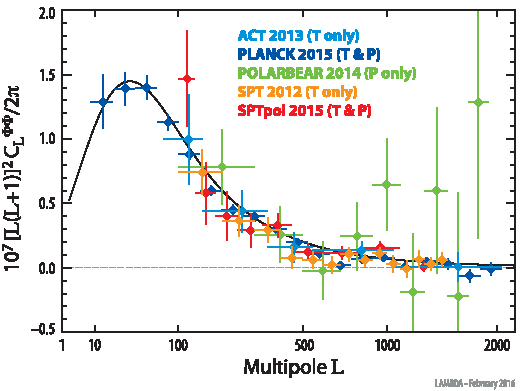
\includegraphics[width=0.85\textwidth]{Chapter1/Images/lensing_power_2016feb}
\caption{Status of CMB lensing measurements as of February 2016. Band powers shown in the plot are from ACT, \textit{Planck} full mission, POLARBEAR, SPT, and SPTPol. The black solid line represents the theoretical lensing power spectrum for the best-fit \gls{LCDM} parameters obtained from the \textit{Planck} 2015 temperature and polarization data. The figure is taken from the Legacy Archive for Microwave Background Data Analysis (LAMBDA) website (\url{http://lambda.gsfc.nasa.gov}). \label{fig:cmb_obs}}
\end{figure}

\myparagraph{Current status of observations}
\gls{CMB} lensing is a fast evolving field of research. The first observational hints of the lensing effects on \gls{CMB}
were found by \cite{Smith2007} and \cite{Hirata2008}, who cross-correlated properly filtered \gls{CMB} maps obtained from
\gls{WMAP} with external \gls{LSS} tracers. On the other hand, the first direct evidence of a preference for a lensed
\gls{CMB} is due to \cite{Reichardt2009} who combined \gls{ACBAR} and \gls{WMAP} data. With the advent of the high
sensitivity small scale \gls{CMB} temperature experiment such as \gls{ACT} \citep{Das2011} and \gls{SPT} 
\citep{Keisler2011}, the \gls{CMB} lensing potential reconstruction has become truly feasible for the first time, with reported detection significance around $\sim4-6\sigma$. The next step forward in \gls{CMB} lensing science has 
been made by the Planck team who detected the \gls{CMB} lensing power spectrum at a significance of about
$25\sigma$ and reconstructed an almost full-sky lensing map using only temperature data 
\cite{Ade2014c}.\footnote{Consider that the \textit{Planck} satellite is as sensitive to \gls{CMB} lensing as \gls{COBE} was to \gls{CMB} temperature fluctuations: $T:\kappa = $ COBE : Planck.} The first \gls{CMB} lensing measurements using polarization data have been recently 
reported by POLARBEAR \citep{Ade2014e}, SPTPol \citep{Story2015}, and \textit{Planck} \citep{PlanckCollaboration2015}: recent measurements are reported in Fig.~\eqref{fig:cmb_obs}.

\subsection{LSS lensing}
\label{sec:lsslens}
CMB photons are not the only ones that experience gravitational deflection by the intervening \gls{LSS}. 
Galaxy photons are also affected by weak lensing which causes (i) the distortion the \emph{shape} of galaxy images, and (ii) a change in their \emph{magnitude} and \emph{size} \citep{Bartelmann2001}: these 
two main effects are at the core of \gls{WL} measurements. Here, we focus on the relationship between the observables and the cosmological signal in \gls{WL}. 

\myparagraph{Shear measurements}
The most common quantity inferred from observations is the shear of galaxy images.
In the weak lensing limit ($|\gamma|,|\kappa|\ll1$), the shear can be directly estimated from the 
\emph{observed ellipticity} $\hat{\epsilon}$ as follows
%
\be
\epsilon = \gamma + \epsilon_{\rm{int}},
\ee
%
where $\epsilon_{\rm{int}}$ is the intrinsic ellipticity of source galaxies, for which current observations 
suggest $\sigma_{\rm{int}} = \sqrt{\langle|\epsilon_{\rm int}|^2\rangle}\simeq 0.4$. Measurement of
galaxy ellipticities are also complicated by several observational systematics such as the point spread 
function of the instrument and the blurring caused by atmosphere which have to be finely controlled.
Also in this case, what the theory predicts is the statistical correlation of galaxy shears, i.e. the shear
power spectrum (or correlation function). The convergence (angular) power spectrum is equivalent to the
shear power spectrum in the weak lensing limit, i.e. $C_{\ell}^{\kappa\kappa}\simeq C_{\ell}^{\gamma\gamma}$. Moreover, radial information can be used to perform a tomographic analysis of the \gls{WL}
signal by measuring the galaxy shear in redshift slices. Considering two redshift bins $i$ and $j$, with 
associated radial distribution of sources $\frac{\diff N_{i,j}}{\diff z}$, we  can write the tomographic 
cross-power spectra in different bins as 
%
\be
\langle \kappa^i_{\ell m}\kappa^j_{\ell' m'}\rangle = \delta^K_{\ell\ell'}\delta^K_{mm'}C^{\kappa^i\kappa^j}_{\ell},
\ee
%
which can be related to theory through \cite{}
%
\be
\label{eq:lens_spectra}
C_{\ell}^{\kappa^i\kappa^j} = 
\begin{cases}
\int_0^{\infty} \diff\chi \frac{W_i^{\kappa}(\chi)W_j^{\kappa}(\chi)}{f_K^2(\chi)} P_{\delta\delta}\biggl(\frac{\ell}{f_K(\chi)}, \chi \biggr) \\
\int_0^{\infty} \frac{\diff z}{H(z)} \frac{W_i^{\kappa}(z)W_j^{\kappa}(z)}{f_K^2(z)}P_{\delta\delta}\biggl(\frac{\ell}{f_K(z)},z \biggr).\\
\end{cases}
\ee
%
We recall that Eq.~\eqref{eq:lens_spectra} assumes both Limber and Born approximations. The observed 
auto-power spectra also include a shot-noise term due to random galaxy shape, 
$C_{\ell}^{\kappa^i\kappa^j} \to C_{\ell}^{\kappa^i\kappa^j} + \delta_{ij}\sigma^2_{\rm int}/\bar{n}_i$, 
where $\bar{n}_i$ is the average number of galaxies per steradian in the $i$-th redshift bin: a large 
number of sources increases the statistics, hence lowering the noise level.
If we decompose the shear into a tangential and cross component as
%
\begin{align}
\gamma_t &\equiv -\text{Re}[\gamma e^{-2i\phi}],\\
\gamma_{\times} &\equiv -\text{Im}[\gamma e^{-2i\phi}],
\end{align}
%
we can obtain a rotationally invariant linear combination of the cross-correlation functions of $\gamma_{\times}$ and $\gamma_t$  as follows:
%
\be
\begin{split}
\xi^{ij}_{\pm}(\theta) &\equiv \langle \gamma_t(0)\gamma_t(\bm{\theta}) \rangle \pm \langle \gamma_{\times}(0)\gamma_{\times}(\bm{\theta}) \rangle \\
&= \frac{1}{2\pi}\int_0^{\infty} \diff\ell\,\ell C_{\ell}^{\kappa^i\kappa^j} J_{0/4}(\ell\theta),
\end{split}
\ee
%
where the Bessel function $J_0$ ($J_4$) refers to the correlation function $\xi_+$ $(\xi_-)$. A common
estimator of the shear correlation function is \citep{}
%
\be
\label{eq:lens_est}
\hat{\xi}_{\pm}(\theta) = \frac{\sum_{ij}w_iw_j [e_t(\theta_i)e_t(\theta_j) \pm e_{\times}(\theta_i)e_{\times}(\theta_j)]}{\sum_{ij}w_iw_j},
\ee
%
where all galaxy pairs $(i,j)$ separated by an angular distance $|\theta_i-\theta_j|\in \theta$ contribute to
the same angular bin with their respective weights $(w_i, w_j)$. 

An important systematic effect that has
an impact on the above estimator is the intrinsic galaxy alignments due to tidal forces \citep{Hirata2004}. 
In fact, Eq.~\eqref{eq:lens_est} estimates $\langle\hat{\xi}_{\pm}\rangle = \xi_{\pm}+\xi_{\pm}^{\rm{II}}+\xi_{\pm}^{\rm{GI}}$, where $\xi_{\pm}^{\rm{II}}$
measures correlation between the intrinsic ellipticities of neighboring galaxies (known as ${\rm{II}}$) and 
$\xi_{\pm}^{\rm{II}}$ is sensitive to correlation between foreground Galaxy Intrinsic ellipticity and 
background galaxy shear (known as ${\rm{GI}}$). The modeling of galaxy alignment is a very active and
debated area of research, see \citet{Kirk2015} for a review. 

Intrinsic alignments represent a potential contaminant also to \gls{CMB} lensing-galaxy lensing cross-correlation measurements, entering the 2-point function as a
$\langle \kappa_{\rm CMB}{\rm I}\rangle$ term. \citet{Hand2015} measured for the first time the 
cross-correlation between the \gls{ACT} \gls{CMB} lensing and the galaxy convergence of \gls{CFHT} Stripe 82 
(CS82) and reported a lower amplitude with respect to the expect signal. \citet{Troxel2014} showed that intrinsic
alignment contamination could account for a $\approx 15\%$ reduction of the observed discrepancy; 
these findings have been later confirmed by \citet{Chisari2015} who modeled the impact of the intrinsic 
alignment with a model based on early-type\footnote{In this context it means \emph{red} galaxies.} galaxy population to 
\gls{CMB} 
lensing measurements, pointing out that at $z\gtrsim 1.2$ alignments remain largely unconstrained. 
\citet{Larsen2015} have considered the impact of intrinsic alignments of spiral galaxies on the \gls{CMB} 
lensing-galaxy lensing cross-correlation using the quadratic alignment model, finding the signal to be
similar in shape with respect to the linear model but with opposite sign, hence it can potentially reduce
the overall impact.

\myparagraph{Magnification bias}
The size amplification is called \emph{magnification} and leads to a fluctuation in the size and the flux of 
individual galaxies. Two competing effects are at play: one one hand \gls{WL} of photons stretches the 
observed area and \emph{dilutes} the number density, on the other it changes the \emph{apparent 
brightness} and allows galaxies in the survey. In a flux-limited survey, the number density of background 
galaxies is expected to be affected through magnification effects due to the foreground galaxy distribution. 
Let us see how.

In presence of lensing the galaxy flux is magnified by $f^{\rm{obs}} = \mu f^s$, where $f^{\rm{obs}}$ and
$f^s$ are is the observed and intrinsic galaxy flux respectively. 
In the \gls{WL} limit it can be shown that $N(>S)$,
the intrinsic counts of sources with observed flux greater than $S$, is related to the cumulative source 
counts $\tilde{N}(>S)$ observed in a given direction through \citep{Bartelmann2001}
%
\be
\tilde{N}(>S,\nver) = \mu^{\alpha-1}(\nver)N(>S).
\ee
%
Here, $\alpha$ is the logarithmic slope of the cumulative number counts of galaxies at the faint end, 
$\alpha=\frac{\diff\log{N(>S)}}{\diff S}|_{S_{\rm min}}$. Thus, if $\alpha > 1$ ($\alpha<1$), the observed number 
density of objects is enhanced (decreased) by lensing: this effect is the so-called 
\emph{magnification (anti-)bias}. Since $|\kappa|\ll 1$, the magnification $\mu$ can be approximated as $\mu \approx 1 + 2(\alpha-1)\kappa$ and the observed number density of galaxies is modulated by the foreground matter distribution as
%
\be
\label{eq:lens_magbias}
\begin{split}
\delta_g^{\rm{obs}}(\nver,z) &\simeq \delta_g^{\rm{cl}}(\nver,z) + 2(\alpha(z)-1)\kappa(\nver,z) \\
&= \delta_g^{\rm cl}(\nver,z) + \delta_g^{\mu}(\nver,z),
\end{split}
\ee
% 
where $\delta_g^{\rm{cl}}(\nver,z)$ is the intrinsic galaxy clustering term.
By substituting in Eq.~\eqref{eq:lens_magbias} the expression for the convergence $\kappa$ - of the sources in the redshift bin around $z_i$ - we get
%
\be
\delta^{\mu}_{\rm g}(\nver,z) = \frac{3\Omega_{\rm m}}{2c}\frac{H_0^2}{H(z)}(1+z)\chi(z) \int_z^{\infty}dz'\,\biggl(1-\frac{\chi(z)}{\chi(z')}\biggr)(\alpha(z')-1)\frac{dN}{dz'}.
\ee
%
Cosmic magnification measurements can be carried out by correlating the angular positions of 
background and foreground galaxy populations (see \citet{Scranton2005,Gonzalez-Nuevo2014}) and by 
counting galaxies \citep{Negrello2010}. Magnification bias can be either a source of information 
\citep{Hildebrandt2013} or a 
nuisance depending on the analysis performed and it can lead to substantial biases if not properly 
accounted for, as shown for \gls{CMB} lensing-galaxy density \citep{Bianchini2015} and \gls{iSW} 
(\gls{CMB} temperature-galaxy density) measurements \citep{LoVerde2007}.
The high-$z$ \gls{DSFG} detected by Herschel have a steep integrated number counts 
at the limiting flux, hence are potentially sensitive to the magnification bias as we will see in Ch.~\eqref{ch:xc1}.



